\documentclass[11pt,a4paper]{article}
% ------------------------------------------------------------
%  Física Moderna — Cuaderno digitalizado (pp. 33–64)
%  Autor de los apuntes: Pedro de la Cruz Castillo
%  Compilar con pdflatex (dos veces, para el índice).
% ------------------------------------------------------------
\usepackage[utf8]{inputenc}
\usepackage[T1]{fontenc}
\usepackage{lmodern}
\usepackage{microtype}
\usepackage[margin=2.3cm,headheight=14pt]{geometry}
\usepackage{amsmath,amssymb,mathtools,esint,cancel}
\usepackage{booktabs,tabularx,array}
\usepackage{enumitem}
\usepackage{xcolor}
\usepackage{tikz}
\usetikzlibrary{arrows.meta,calc,decorations.pathmorphing,patterns,3d}
\usepackage{pgfplots}
\pgfplotsset{compat=1.16}
\usepackage[most]{tcolorbox}
\usepackage{titlesec}
\usepackage{fancyhdr}
\usepackage[hidelinks]{hyperref}
\usepackage{float}

% --- Idioma (sin babel-spanish): nombres en castellano ---
\renewcommand{\contentsname}{Índice}
\renewcommand{\figurename}{Figura}
\renewcommand{\tablename}{Tabla}

% --- Colores y estilo ---
\definecolor{azul}{RGB}{31,78,121}
\definecolor{obsfondo}{RGB}{255,248,230}
\definecolor{obsborde}{RGB}{214,140,30}
\definecolor{gris}{RGB}{110,110,110}

\titleformat{\section}{\Large\bfseries\color{azul}}{\thesection.}{0.6em}{}
\titleformat{\subsection}{\large\bfseries}{\thesubsection}{0.6em}{}
\titleformat{\subsubsection}{\normalsize\bfseries}{}{0em}{}
\setcounter{secnumdepth}{2}

\pagestyle{fancy}
\fancyhf{}
\fancyhead[L]{\small\color{gris}Física Moderna}
\fancyhead[R]{\small\color{gris}\thesection.\ \leftmark}
\fancyfoot[C]{\thepage}
\renewcommand{\headrulewidth}{0.4pt}
\renewcommand{\sectionmark}[1]{\markboth{#1}{}}

\setlist{itemsep=2pt,topsep=4pt}
\setlength{\parindent}{0pt}
\setlength{\parskip}{5pt}

% --- Observaciones (añadidos, no forman parte del cuaderno) ---
\newtcolorbox{obs}{enhanced,breakable,colback=obsfondo,colframe=obsborde,
  boxrule=0.6pt,arc=2pt,left=6pt,right=6pt,top=4pt,bottom=4pt,
  fonttitle=\bfseries\small,coltitle=black,
  title={Observación},attach title to upper={\ }}

% --- Página del cuaderno en el margen ---
\newcommand{\pag}[1]{\marginpar{\footnotesize\color{gris}p.~#1}}
\newcommand{\pags}[1]{{\normalfont\small\color{gris}(pp.~#1)}}

% --- Atajos ---
\newcommand{\ii}{\hat{\imath}}
\newcommand{\jj}{\hat{\jmath}}
\newcommand{\kk}{\hat{k}}
\newcommand{\vect}[1]{\vec{#1}}
\newcommand{\Ep}{\mathcal{E}}
\DeclareMathOperator{\sen}{sen}

\begin{document}

\begin{titlepage}
  \centering
  \vspace*{3cm}
  {\Huge\bfseries\color{azul} Física Moderna\par}
  \vspace{0.6cm}
  {\Large Cuaderno digitalizado\par}
  \vspace{0.4cm}
  {\large Páginas 33–64 del cuaderno\par}
  \vspace{2cm}
  {\large Pedro de la Cruz Castillo\par}
  \vfill
  \begin{minipage}{0.85\textwidth}
  \small
  Transcripción fiel del cuaderno de clase, ordenada por temas. En el margen se indica la
  página original de cada parte. Los recuadros
  \tcbox[on line,colback=obsfondo,colframe=obsborde,boxrule=0.5pt,arc=1pt,
  left=2pt,right=2pt,top=0pt,bottom=0pt]{\textbf{\small Observación}}
  son añadidos posteriores (aclaraciones y correcciones), no forman parte del cuaderno.
  \end{minipage}
  \vspace{1.5cm}
\end{titlepage}

\tableofcontents
\newpage
% ============================================================
\section{Ecuaciones de Maxwell \pags{33}}
% ============================================================

\begin{center}
\renewcommand{\arraystretch}{1.6}
\begin{tabular}{@{}lll@{}}
\toprule
\textbf{Ley} & \textbf{Forma integral} & \textbf{Forma diferencial}\\
\midrule
(1) Gauss para $\vec E$ & $\displaystyle\oint \vec E\cdot d\vec S=\frac{q}{\varepsilon_0}$ & $\nabla\cdot\vec E=\dfrac{\rho}{\varepsilon_0}$\\
(2) Gauss para $\vec B$ & $\displaystyle\oint \vec B\cdot d\vec S=0$ & $\nabla\cdot\vec B=0$\\
(3) Faraday--Henry & $\displaystyle\oint \vec E\cdot d\vec l=-\frac{d}{dt}\int\vec B\cdot d\vec S$ & $\nabla\times\vec E=-\dfrac{\partial\vec B}{\partial t}$\\
(4) Ampère--Maxwell & $\displaystyle\oint \vec B\cdot d\vec l=\mu_0 i+\mu_0\varepsilon_0\frac{d}{dt}\int\vec E\cdot d\vec S$ & $\nabla\times\vec B=\mu_0\vec J+\mu_0\varepsilon_0\dfrac{\partial\vec E}{\partial t}$\\
\bottomrule
\end{tabular}
\end{center}

\textbf{Interpretación:}
\begin{itemize}
  \item Ecuaciones (1) y (2): existencia o no de cargas eléctricas o magnéticas.
  \item Ecuaciones (3) y (4): cambio de $\vec B$ genera $\vec E$; cambio de $\vec E$ genera $\vec B$.
\end{itemize}

% ============================================================
\section{Ondas electromagnéticas (OEM) \pags{33--34}}
% ============================================================

\subsection{Ecuación de onda}
\[
\frac{\partial^2\xi}{\partial t^2}=v^2\,\frac{\partial^2\xi}{\partial x^2}
\qquad \xi:\ \text{perturbación que se propaga.}
\]

Tomamos el campo E/M:
\[
E_x=0,\quad E_y=E,\quad E_z=0;\qquad B_x=0,\quad B_y=0,\quad B_z=B.
\]
Verifiquemos si este campo E/M satisface la ecuación de onda. Haremos el análisis en el vacío: $\rho=0$, $\vec J=0$.

\textbf{Ecuación (1):}
\[
\nabla\cdot\vec E=\frac{\rho}{\varepsilon_0}\ \rightarrow\
\frac{\partial E_x}{\partial x}+\frac{\partial E_y}{\partial y}+\frac{\partial E_z}{\partial z}=0
\ \rightarrow\ \frac{\partial E}{\partial y}=0 \qquad (a)
\]

\textbf{Ecuación (2):}
\[
\nabla\cdot\vec B=0\ \rightarrow\ \frac{\partial B}{\partial z}=0 \qquad (b)
\]

\textbf{Ecuación (3):}
\[
\nabla\times\vec E=-\frac{\partial\vec B}{\partial t}:\qquad
\begin{vmatrix}\ii&\jj&\kk\\ \partial_x&\partial_y&\partial_z\\ 0&E&0\end{vmatrix}
=-\frac{\partial}{\partial t}\left(B\,\kk\right)
\]
\[
-\frac{\partial E}{\partial z}\,\ii+\frac{\partial E}{\partial x}\,\kk=-\frac{\partial B}{\partial t}\,\kk
\ \rightarrow\
\frac{\partial E}{\partial z}=0\quad(c_1),\qquad
\frac{\partial E}{\partial x}=-\frac{\partial B}{\partial t}\quad(c_2)
\]

\textbf{Ecuación (4):}
\[
\nabla\times\vec B=\varepsilon_0\mu_0\frac{\partial\vec E}{\partial t}:\qquad
\begin{vmatrix}\ii&\jj&\kk\\ \partial_x&\partial_y&\partial_z\\ 0&0&B\end{vmatrix}
=\varepsilon_0\mu_0\frac{\partial}{\partial t}\left(E\,\jj\right)
\]
\[
\frac{\partial B}{\partial y}\,\ii-\frac{\partial B}{\partial x}\,\jj=\varepsilon_0\mu_0\frac{\partial E}{\partial t}\,\jj
\ \rightarrow\
\frac{\partial B}{\partial y}=0\quad(d_1),\qquad
\frac{\partial B}{\partial x}=-\varepsilon_0\mu_0\frac{\partial E}{\partial t}\quad(d_2)
\]

\textbf{Derivamos $(c_2)$ por $x$ y $(d_2)$ por $t$:}
\[
\frac{\partial^2E}{\partial x^2}=-\frac{\partial^2B}{\partial x\,\partial t},\qquad
\frac{\partial^2B}{\partial t\,\partial x}=-\varepsilon_0\mu_0\frac{\partial^2E}{\partial t^2}
\ \Rightarrow\
\boxed{\frac{\partial^2E}{\partial t^2}=\frac{1}{\varepsilon_0\mu_0}\frac{\partial^2E}{\partial x^2}}
\]

\textbf{Derivamos $(c_2)$ por $t$ y $(d_2)$ por $x$:}
\[
\boxed{\frac{\partial^2B}{\partial t^2}=\frac{1}{\varepsilon_0\mu_0}\frac{\partial^2B}{\partial x^2}}
\]

\subsection{Velocidad de propagación}
\[
c=\frac{1}{\sqrt{\varepsilon_0\mu_0}}=2{,}999\ldots\times10^{8}\ \text{m/s}
\qquad\text{(velocidad de la luz en el vacío).}
\]

\subsection{Características de las OEM}
\begin{itemize}
  \item $\vec E\perp\vec B$
  \item $(\vec E\times\vec B)\parallel\vec k$ \quad ($\vec k$: vector de onda)
  \item $B=E/c$
\end{itemize}

\subsection{Energía}
Densidad de energía:
\[
u=u_E+u_B=\frac{\varepsilon_0E^2}{2}+\frac{B^2}{2\mu_0}
=\frac{\varepsilon_0E^2}{2}+\frac{1}{2\mu_0}\left(\frac{E}{1/\sqrt{\varepsilon_0\mu_0}}\right)^2
=\frac{\varepsilon_0E^2}{2}+\frac{\varepsilon_0E^2}{2}=\varepsilon_0E^2
\]

\textbf{Intensidad} (energía que atraviesa una superficie $S$):
\[
I=c\,\varepsilon_0E^2=c\,u
\]

\begin{obs}
Esta es la intensidad instantánea. Para una onda armónica $E=E_0\sen(kx-\omega t)$ el promedio
temporal es $\langle I\rangle=\tfrac12 c\,\varepsilon_0E_0^2$, que es el valor que suele pedirse en problemas.
\end{obs}

\textbf{Vector de Poynting ($\vec\Pi$):}
\[
\vec\Pi=c^2\varepsilon_0\,(\vec E\times\vec B),\qquad
|\vec\Pi|=c^2\varepsilon_0\,E\,\frac{E}{c}=I,\qquad
\text{dirección: }\vec E\times\vec B\parallel\vec k.
\]

\begin{obs}
Como $c^2\varepsilon_0=1/\mu_0$, también se escribe $\vec\Pi=\frac{1}{\mu_0}\vec E\times\vec B$ (en muchos libros se denota $\vec S$).
\end{obs}

\textbf{Densidad de la cantidad de movimiento:}
\[
\vec p=\varepsilon_0\,(\vec E\times\vec B)
\]

\subsection{Fuentes de radiación}
\begin{itemize}
  \item \textbf{Dipolo eléctrico oscilante:} $\vec p=q\,\vec a$ (vector de $-q$ a $+q$); oscilante: $p=p_0\sen\omega t$.
  \item \textbf{Dipolo magnético oscilante:} espira de área $S$ con corriente $i$, $|\vec\mu|=iS$; oscilante: $\mu=\mu_0\sen\omega t$.
  \item \textbf{Carga acelerada.}
\end{itemize}

\textbf{Criterio:} un objeto emite OEM si $\displaystyle\oint\vec\Pi\cdot d\vec S\neq0$.

\begin{figure}[H]
\centering
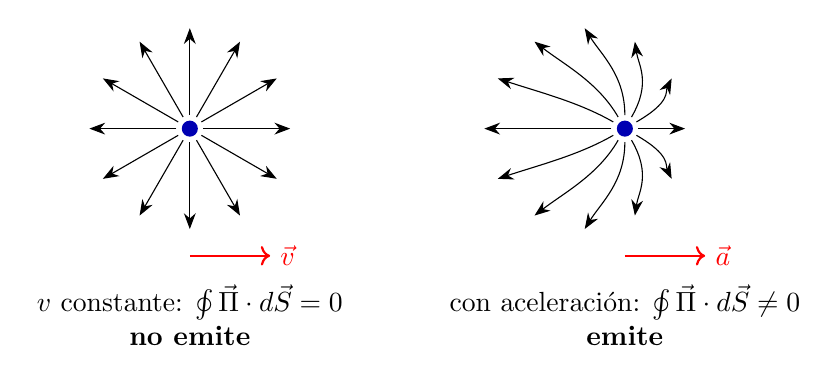
\begin{tikzpicture}[scale=0.85]
  % carga con v constante
  \begin{scope}
    \fill[blue!70!black] (0,0) circle (0.12);
    \foreach \a in {0,30,...,330}
      \draw[-{Stealth[length=2mm]}] (\a:0.2) -- (\a:1.5);
    \draw[->,thick,red] (0,-1.9) -- (1.2,-1.9) node[right]{$\vec v$};
    \node at (0,-2.6) {$v$ constante: $\oint\vec\Pi\cdot d\vec S=0$};
    \node at (0,-3.1) {\textbf{no emite}};
  \end{scope}
  % carga acelerada
  \begin{scope}[xshift=6.5cm]
    \fill[blue!70!black] (0,0) circle (0.12);
    \foreach \a in {0,30,...,330}
      \draw[-{Stealth[length=2mm]}] (\a:0.2) .. controls (\a:0.8) and ($(\a:1.1)+(-0.35,0)$) .. ($(\a:1.5)+(-0.6,0)$);
    \draw[->,thick,red] (0,-1.9) -- (1.2,-1.9) node[right]{$\vec a$};
    \node at (0,-2.6) {con aceleración: $\oint\vec\Pi\cdot d\vec S\neq0$};
    \node at (0,-3.1) {\textbf{emite}};
  \end{scope}
\end{tikzpicture}
\caption{Líneas de campo de una carga con velocidad constante (los campos se mueven con la carga) y de una carga acelerada (las líneas se curvan).}
\end{figure}

\textbf{Fórmula de Larmor} (potencia de radiación de una carga acelerada):
\[
\frac{d\Ep}{dt}=\frac{q^2a^2}{6\pi\varepsilon_0c^3}
\]

% ============================================================
\section{Radiación del cuerpo negro \pags{34--36}}
% ============================================================

\subsection{Radiación térmica}
\begin{itemize}
  \item Todos los cuerpos emiten radiación.
  \item Los más calientes emiten radiación de mayor intensidad.
  \item Emiten en diferentes frecuencias con diferente intensidad (espectro).
  \item También absorben.
  \item Mientras más absorben una radiación, más emiten esa radiación.
\end{itemize}

\textbf{Poder emisivo $\Ep_T(\nu)$} (o radiancia $R_T(\nu)$), función de la temperatura $T$ y la frecuencia $\nu$:
es la energía de frecuencia $\nu$ que emite el cuerpo que está a temperatura $T$, a través de su superficie,
por unidad de área y por unidad de tiempo. Unidades: $\dfrac{\text{energía}}{\text{área}\cdot t}$.

\textbf{Poder absorbente $A_T(\nu)$:} indica qué porción de la energía de frecuencia $\nu$ absorbe el cuerpo,
que está a temperatura $T$, por unidad de área y por unidad de tiempo.

\textbf{Cuerpo negro:} el que absorbe toda la radiación incidente: $A_T(\nu)=1$.

\subsection{Ley de Kirchhoff}
Para cualquier cuerpo con $\Ep_T(\nu)$ y $A_T(\nu)$ (a la misma $T$ y $\nu$):
\[
\frac{\Ep_T(\nu)}{A_T(\nu)}=\text{const}=\varepsilon_T(\nu)
\]
\begin{itemize}
  \item Si tenemos un cuerpo negro, $A_T(\nu)=1\ \rightarrow\ \Ep_T(\nu)/1=\varepsilon_T(\nu)$.
        Entonces $\varepsilon_T(\nu)$ es el \textbf{poder emisivo del cuerpo negro}.
  \item Si tenemos un cuerpo no negro, $A_T(\nu)<1\ \rightarrow\ \Ep_T(\nu)=A_T(\nu)\,\varepsilon_T(\nu)\ \rightarrow\ \Ep_T(\nu)<\varepsilon_T(\nu)$.
\end{itemize}
O sea, el cuerpo negro tiene la mayor capacidad de emitir.

\subsection{Ecuación dimensional de $\Ep_T(\nu)$}
\textbf{Espectro discreto} (líneas en $\nu_1,\nu_2,\nu_3$):
\[
\Ep_T=\Ep_T(\nu_1)+\Ep_T(\nu_2)+\Ep_T(\nu_3)\qquad\left[\frac{\text{energía}}{\text{área}\cdot t}\right]
\]
\textbf{Espectro continuo:}
\[
\Ep_T=\int\Ep_T(\nu)\,d\nu\quad\left[\frac{\text{energía}}{\text{área}\cdot t}\right],\qquad
\Ep_T(\nu)\quad\left[\frac{\text{energía}}{\text{área}\cdot t\cdot\Delta\nu}\right]
\]

\subsection{Leyes de radiación del cuerpo negro (encontradas empíricamente)}

\begin{figure}[H]
\centering
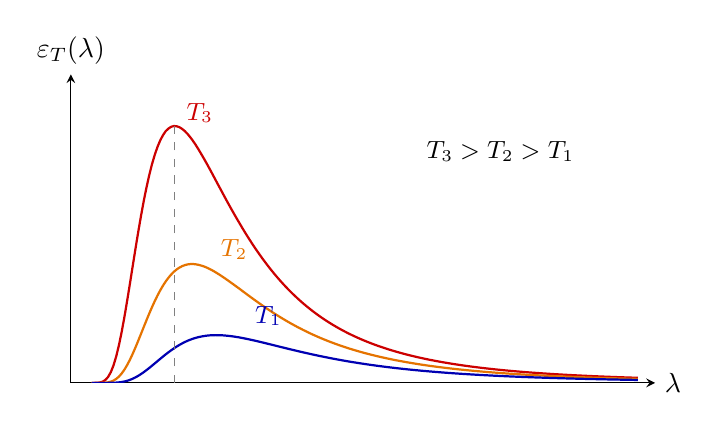
\begin{tikzpicture}
\begin{axis}[width=9cm,height=5.5cm,axis lines=left,xlabel={$\lambda$},ylabel={$\varepsilon_T(\lambda)$},
  xtick=\empty,ytick=\empty,xmin=0,xmax=3.4,ymin=0,ymax=1.2,samples=200,domain=0.12:3.3,
  every axis x label/.style={at={(ticklabel* cs:1)},anchor=west},
  every axis y label/.style={at={(ticklabel* cs:1)},anchor=south}]
  \addplot[thick,red!80!black]   {11.45*x^(-5)/(exp(3.0/x)-1)};
  \addplot[thick,orange!90!black]{11.45*x^(-5)/(exp(3.5/x)-1)};
  \addplot[thick,blue!70!black]  {11.45*x^(-5)/(exp(4.2/x)-1)};
  \node[font=\small,red!80!black] at (axis cs:0.75,1.05) {$T_3$};
  \node[font=\small,orange!90!black] at (axis cs:0.95,0.52) {$T_2$};
  \node[font=\small,blue!70!black] at (axis cs:1.15,0.26) {$T_1$};
  \draw[dashed,gray] (axis cs:0.604,0) -- (axis cs:0.604,1.0);
  \node[font=\small,gray,below] at (axis cs:0.604,0) {$\lambda_{\text{máx}}$};
  \node[font=\small] at (axis cs:2.5,0.9) {$T_3>T_2>T_1$};
\end{axis}
\end{tikzpicture}
\caption{Curvas experimentales del espectro del cuerpo negro: a mayor temperatura el pico es más alto y se desplaza a $\lambda$ menores.}
\end{figure}

\textbf{Ley de Stefan--Boltzmann:} $\Ep_T\sim T^4$
\[
\Ep_T=\sigma T^4,\qquad \Ep_T=\int\varepsilon_T(\lambda)\,d\lambda
\]
$\Ep_T$: poder emisivo total (el área bajo la curva $\varepsilon_T(\lambda)$).

\textbf{Ley de desplazamiento de Wien:} $\lambda_{\text{máx}}\sim 1/T$
\[
\lambda_{\text{máx}}=\frac{b}{T}
\]

\begin{obs}
Valores de referencia: $\sigma=5{,}67\times10^{-8}\ \text{W}/(\text{m}^2\cdot\text{K}^4)$ y $b=2{,}898\times10^{-3}\ \text{m}\cdot\text{K}$.
\end{obs}

\subsection{El problema}
Los físicos intentaron deducir teóricamente una expresión para la curva y llegaron a resultados
contradictorios: la fórmula de \textbf{Rayleigh--Jeans} coincide con la curva solo a bajas frecuencias y luego
se dispara; la de \textbf{Wien} coincide solo a altas frecuencias.

\begin{figure}[H]
\centering
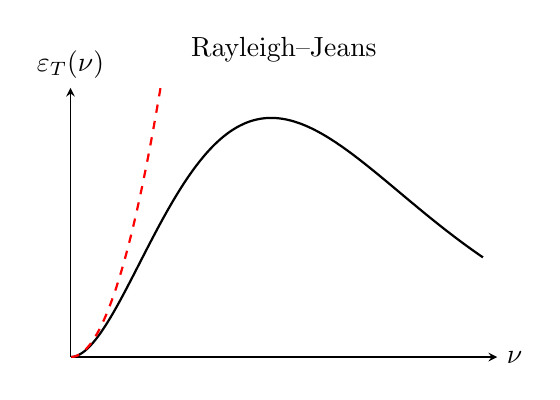
\begin{tikzpicture}
\begin{axis}[width=7cm,height=5cm,axis lines=left,xlabel={$\nu$},ylabel={$\varepsilon_T(\nu)$},
  xtick=\empty,ytick=\empty,xmin=0,xmax=6,ymin=0,ymax=1.6,samples=150,domain=0.01:5.8,
  every axis x label/.style={at={(ticklabel* cs:1)},anchor=west},
  every axis y label/.style={at={(ticklabel* cs:1)},anchor=south},title={Rayleigh--Jeans}]
  \addplot[thick] {x^3/(exp(x)-1)};
  \addplot[thick,dashed,red,domain=0.01:1.3] {x^2};
\end{axis}
\end{tikzpicture}\hspace{0.5cm}
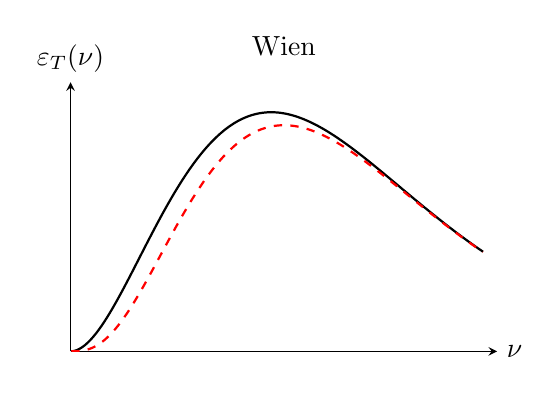
\begin{tikzpicture}
\begin{axis}[width=7cm,height=5cm,axis lines=left,xlabel={$\nu$},ylabel={$\varepsilon_T(\nu)$},
  xtick=\empty,ytick=\empty,xmin=0,xmax=6,ymin=0,ymax=1.6,samples=150,domain=0.01:5.8,
  every axis x label/.style={at={(ticklabel* cs:1)},anchor=west},
  every axis y label/.style={at={(ticklabel* cs:1)},anchor=south},title={Wien}]
  \addplot[thick] {x^3/(exp(x)-1)};
  \addplot[thick,dashed,red] {x^3*exp(-x)};
\end{axis}
\end{tikzpicture}
\caption{Curva experimental (continua) frente a las fórmulas teóricas (discontinuas).}
\end{figure}

\begin{obs}
La divergencia de Rayleigh--Jeans a altas frecuencias se conoce como \emph{catástrofe ultravioleta}.
\end{obs}

\subsection{Idea de Planck (1900)}
\begin{itemize}
  \item La radiación se emite en porciones aisladas (cuantos).
  \item La energía de cada cuanto es $E\sim\nu$:\quad $E=h\nu$.
\end{itemize}

\textbf{Fórmula de Planck:}
\[
\boxed{\varepsilon_T(\nu)=\frac{2\pi h\nu^3}{c^2\left(e^{h\nu/k_BT}-1\right)}}
\]

% ============================================================
\section{Efecto fotoeléctrico \pags{36}}
% ============================================================

Extracción de e$^-$ de la superficie del metal por acción de la luz (\emph{photo} $\rightarrow$ luz;
\emph{eléctrico} $\rightarrow$ electrones).

\textbf{Hertz (1887):} experimento con descargador de chispas ($\approx5000$~V / 2000~V). La luz que incide
sobre el metal arranca electrones con velocidad $v_0$ y aparece una corriente $I$.

Se hicieron deducciones (clásicas) que llevaron a resultados contradictorios:
\begin{itemize}
  \item $v_0$ depende de $I$.
  \item El e$^-$ debe tardar en salir (inercia del efecto fotoeléctrico).
\end{itemize}

\subsection{Einstein}
Plantea la naturaleza corpuscular de la radiación: la radiación está formada por partículas (cuantos, fotones).
La energía de cada cuanto es $E=h\nu$.

Efecto fotoeléctrico: choque del fotón con el e$^-$.
\[
h\nu=\phi+\frac{mv_0^2}{2}+(\text{otros procesos})
\qquad\Rightarrow\qquad
\boxed{h\nu=\phi+\frac{mv_{0\,\text{máx}}^2}{2}}
\]
$\phi$: trabajo de salida del metal (función trabajo del metal).

\subsection{Arreglo experimental}
Tubo al vacío con cátodo C (iluminado) y ánodo A, fuente de voltaje variable $V$ y amperímetro.

\begin{figure}[H]
\centering
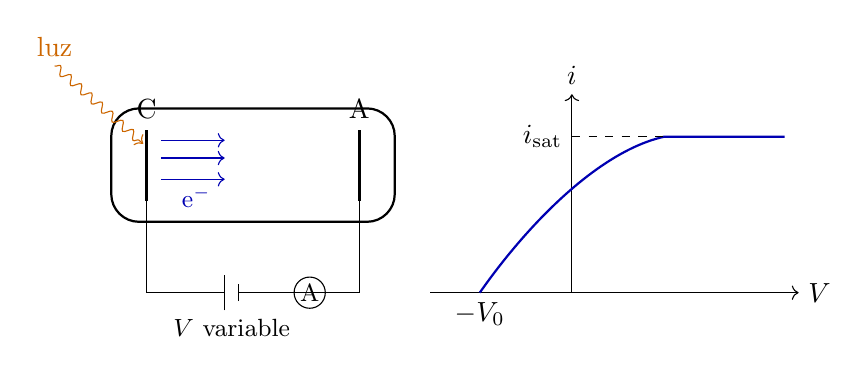
\begin{tikzpicture}[scale=0.9]
  % tubo
  \draw[thick,rounded corners=10pt] (0,0) rectangle (4,1.6);
  \draw[very thick] (0.5,0.3) -- (0.5,1.3) node[above]{C};
  \draw[very thick] (3.5,0.3) -- (3.5,1.3) node[above]{A};
  \draw[->,decorate,decoration={snake,amplitude=1.5pt,segment length=5pt},orange!80!black] (-0.8,2.2) -- (0.45,1.1) node[pos=0,above]{luz};
  \foreach \y in {0.6,0.9,1.15} \draw[->,blue!70!black] (0.7,\y) -- (1.6,\y);
  \node[blue!70!black,font=\small] at (1.2,0.35) {e$^-$};
  % circuito
  \draw (0.5,0.3) -- (0.5,-1) -- (1.6,-1);
  \draw (2.4,-1) -- (3.5,-1) -- (3.5,0.3);
  \draw (1.6,-1.25) -- (1.6,-0.75); \draw (1.8,-1.12) -- (1.8,-0.88);
  \draw (1.8,-1) -- (2.4,-1);
  \node[font=\small] at (1.7,-1.5) {$V$ variable};
  \draw (2.8,-1) circle (0.22) node{\small A};
  % curva I-V
  \begin{scope}[xshift=6.5cm,yshift=-1cm]
    \draw[->] (-2,0) -- (3.2,0) node[right]{$V$};
    \draw[->] (0,0) -- (0,2.8) node[above]{$i$};
    \draw[thick,blue!70!black] (-1.3,0) .. controls (-0.6,1.0) and (0.4,2.0) .. (1.3,2.2) -- (3,2.2);
    \draw[dashed] (0,2.2) node[left]{$i_{\text{sat}}$} -- (1.3,2.2);
    \node[below] at (-1.3,0) {$-V_0$};
  \end{scope}
\end{tikzpicture}
\caption{Arreglo experimental y curva corriente--voltaje: la corriente se satura en $i_{\text{sat}}$ y se anula en el potencial de frenado $-V_0$.}
\end{figure}

\begin{obs}
El potencial de frenado da directamente la energía cinética máxima: $eV_0=\tfrac12mv_{0\,\text{máx}}^2$, de modo que
$eV_0=h\nu-\phi$. Graficando $V_0$ vs.\ $\nu$ se obtiene una recta de pendiente $h/e$.
\end{obs}

\textbf{Ejemplo del cuaderno:} supongamos que en cada segundo inciden 30 fotones y se desprenden 3 e$^-$ por segundo.
Los 3 e$^-$ recorren el espacio en 0,3~s. Ahora aumento el voltaje $V$ $\rightarrow$ recorren en 0,2~s. Pero el número de
e$^-$/s que llega al ánodo A sigue siendo el mismo (por eso la corriente se satura).

\subsection{Intensidad en la naturaleza corpuscular}
\[
I=N\,h\nu,\qquad N=\frac{\#\ \text{fotones}}{\text{área}\cdot t}
\]
% ============================================================
\section{Efecto Compton \pags{37--38}}
% ============================================================

Dispersión de rayos X por cuerpos ligeros como el grafito y la parafina. «Ligero»: los e$^-$ de los últimos
niveles atómicos están débilmente ligados al átomo (casi libres). Un haz de longitud de onda $\lambda$ incide
sobre el material y sale dispersado un haz $\lambda'$ a un ángulo $\theta$.

\textbf{Teoría clásica:} la onda es la propagación de oscilaciones; al llegar al cuerpo (sistema de cargas)
genera oscilaciones en la misma frecuencia, que luego el cuerpo emite como el haz dispersado.

Pero, experimentalmente, $\lambda'\neq\lambda$:
\[
\lambda'=\lambda+\lambda_C\,(1+\cos\theta),\qquad \lambda_C:\ \text{longitud de onda Compton }(2{,}43\times10^{-12}\ \text{m}).
\]

\begin{obs}
Aquí el cuaderno tiene un desliz de signo: la fórmula correcta es $\lambda'=\lambda+\lambda_C(1-\cos\theta)$, como se
obtiene al final de la deducción (p.~38). Con el «$+$», a $\theta=0$ habría corrimiento, lo cual es falso.
\end{obs}

\textbf{Teoría moderna:} choque de un fotón con un electrón (el e$^-$ antes del choque se considera en reposo).

\begin{figure}[H]
\centering
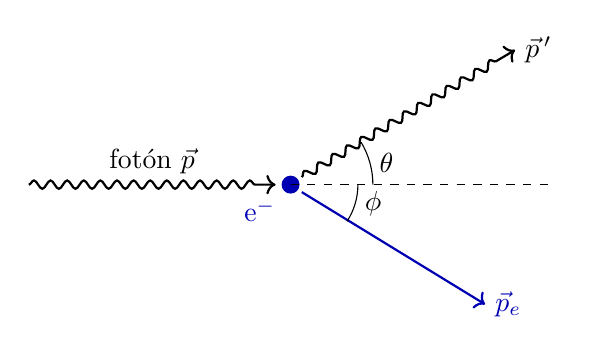
\begin{tikzpicture}[scale=0.95]
  \draw[->,thick,decorate,decoration={snake,amplitude=1.5pt,segment length=6pt,post length=2mm}] (-3.5,0) -- (-0.2,0) node[midway,above]{fotón $\vec p$};
  \fill[blue!70!black] (0,0) circle (0.12) node[below left=2pt]{e$^-$};
  \draw[dashed] (0,0) -- (3.5,0);
  \draw[->,thick,decorate,decoration={snake,amplitude=1.5pt,segment length=6pt,post length=2mm}] (0.15,0.1) -- (3,1.8) node[right]{$\vec p\,'$};
  \draw[->,thick,blue!70!black] (0.15,-0.1) -- (2.6,-1.6) node[right]{$\vec p_e$};
  \draw (1.1,0) arc (0:31:1.1) node[midway,right]{$\theta$};
  \draw (0.9,0) arc (0:-33:0.9) node[midway,right]{$\phi$};
\end{tikzpicture}
\caption{Choque fotón--electrón en el efecto Compton.}
\end{figure}

Deben cumplirse las leyes de los choques:
\begin{itemize}
  \item Conservación de $\vec p$.
  \item Conservación de $E$.
\end{itemize}

\subsection{Teoría de la relatividad especial}
\textbf{Postulados:}
\begin{itemize}
  \item El espacio y el tiempo no son absolutos.
  \item La velocidad de la luz en el vacío es igual en todos los sistemas inerciales.
\end{itemize}

\textbf{Transformaciones de Galileo} ($S'$ se mueve con velocidad $v$ a lo largo de $x$):
\[
x'=x-vt,\quad y'=y,\quad z'=z,\quad t'=t;\qquad V'_x=V_x-v,\quad a'_x=a_x
\]

\textbf{Transformaciones de Lorentz:}
\[
x'=\frac{x-vt}{\sqrt{1-v^2/c^2}},\quad y'=y,\quad z'=z,\quad t'=\frac{t-xv/c^2}{\sqrt{1-v^2/c^2}}
\]

\textbf{$c$ es la misma en todos los sistemas inerciales:} un observador en reposo y otro que se mueve con $v$
miden la misma $c$ para la luz de una fuente (no $c+v$).
\[
E=mc^2,\qquad E=m_0c^2+E_K,\qquad E=c\sqrt{m_0^2c^2+p^2},\qquad m=\frac{m_0}{\sqrt{1-v^2/c^2}}
\]
Más adelante demostraremos: $p=h/\lambda$ (para el fotón).

\subsection{Deducción}
Conservación del momento: $\vec p+0=\vec p\,'+\vec p_e$.

En $x$:
\[
p=p'\cos\theta+p_e\cos\phi\ \rightarrow\ \frac{h}{\lambda}=\frac{h}{\lambda'}\cos\theta+p_e\cos\phi \qquad (1)
\]
En $y$:
\[
0=p_e\sen\phi-\frac{h}{\lambda'}\sen\theta \qquad (2)
\]
Energía:
\[
\frac{hc}{\lambda}+m_0c^2=\frac{hc}{\lambda'}+c\sqrt{m_0^2c^2+p_e^2} \qquad (3)
\]
Se obtiene:
\[
\boxed{\lambda'=\lambda+\frac{h}{m_0c}\,(1-\cos\theta)}
\]

\begin{obs}
El paso intermedio (omitido en el cuaderno): de (1) y (2), elevar al cuadrado y sumar para eliminar $\phi$
$\Rightarrow p_e^2=p^2+p'^2-2pp'\cos\theta$; luego despejar $p_e^2$ de (3) e igualar.
Así, $\lambda_C=h/(m_0c)=2{,}43\times10^{-12}$~m.
\end{obs}

% ============================================================
\section{Átomo de Bohr \pags{38}}
% ============================================================

\textbf{Modelo de Thomson (1904):} «pudín de pasas».\qquad
\textbf{Rutherford (1911):} modelo planetario.

Intrigó a los físicos:
\begin{itemize}
  \item El espectro de emisión de los elementos (átomo aislado) era discreto.
  \item El e$^-$ en el átomo es carga acelerada: debe emitir radiación, pierde energía, disminuye paulatinamente
        el radio de su órbita y debe caer en el núcleo. Pero no es así.
\end{itemize}

\subsection{Postulados de Bohr}
\begin{enumerate}
  \item Los electrones giran en el átomo alrededor del núcleo en órbitas circulares y sin emitir radiación.
  \item Solo son posibles aquellas órbitas en las que el momento angular del electrón es múltiplo de $\hbar$:
        $L=n\hbar$ \ ($\hbar=h/2\pi$), \ $n=1,2,3,\ldots$
  \item Si un electrón pasa de un nivel de energía $E_A$ a un nivel de energía menor $E_B$, entonces emite un
        fotón, cuya frecuencia se calcula a partir de la fórmula: $E_A-E_B=h\nu$.
\end{enumerate}

\subsection{Ejemplo: radio de las órbitas del átomo de H}
\[
F=\frac{1}{4\pi\varepsilon_0}\frac{e^2}{r^2}=m\frac{v^2}{r}\cdot\frac{mr^2}{mr^2}
\ \Rightarrow\
\frac{e^2}{4\pi\varepsilon_0r^2}=\frac{(n\hbar)^2}{mr^3}
\]
\[
\boxed{r=\frac{4\pi\varepsilon_0\hbar^2n^2}{me^2}},\qquad n=1,2,3,\ldots\qquad n=1\ \rightarrow\ r_1=a=0{,}53\ \text{Å}
\]

\subsection{Ejemplo: energía del átomo de H}
\[
E=E_K+E_P=\frac{mv^2}{2}+\frac{(+e)(-e)}{4\pi\varepsilon_0r}
=\frac12\left(\frac{e^2}{4\pi\varepsilon_0r}\right)-\frac{e^2}{4\pi\varepsilon_0r}=-\frac{e^2}{8\pi\varepsilon_0r}
\]
\[
E=\frac{-e^2}{8\pi\varepsilon_0\left(\dfrac{4\pi\varepsilon_0\hbar^2n^2}{me^2}\right)}
\ \Rightarrow\
\boxed{E=-\frac{me^4}{32\pi^2\varepsilon_0^2\hbar^2n^2}}
\]

\begin{minipage}{0.45\textwidth}
\centering
\begin{tabular}{cc}
\toprule
$n$ & $E_n$\\
\midrule
1 & $-13{,}6$ eV\\
2 & $-13{,}6/2^2=-3{,}4$ eV\\
3 & $-13{,}6/3^2=-1{,}51$ eV\\
\bottomrule
\end{tabular}
\end{minipage}\hfill
\begin{minipage}{0.5\textwidth}
\centering
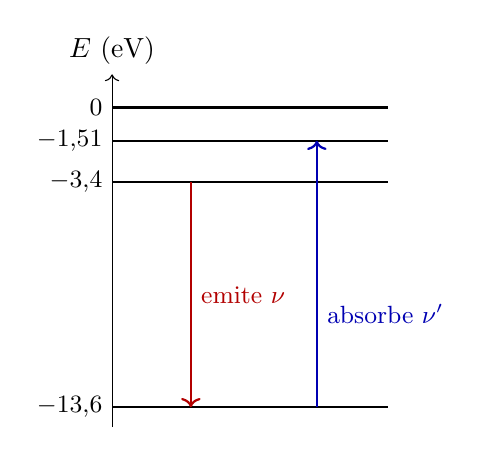
\begin{tikzpicture}[yscale=0.28]
  \draw[->] (0,-14.5) -- (0,1.5) node[above]{$E$ (eV)};
  \foreach \e/\l in {0/0,-1.51/{-1{,}51},-3.4/{-3{,}4},-13.6/{-13{,}6}}
    {\draw[thick] (0,\e) -- (3.5,\e); \node[left,font=\small] at (0,\e) {$\l$};}
  \draw[->,red!70!black,thick] (1,-3.4) -- (1,-13.6) node[midway,right,font=\small]{emite $\nu$};
  \draw[->,blue!70!black,thick] (2.6,-13.6) -- (2.6,-1.51) node[pos=0.35,right,font=\small]{absorbe $\nu'$};
\end{tikzpicture}
\end{minipage}

% ============================================================
\section{Propiedades ondulatorias de la materia \pags{39--40}}
% ============================================================

\textbf{De Broglie:} las partículas tienen propiedades ondulatorias. Para comprobarlo, experimento.
Difracción: característico de ondas (haz $\rightarrow$ rendija $\rightarrow$ pantalla con franjas).

\textbf{Huygens:} cada punto de un frente de onda se comporta como una fuente puntual de ondas secundarias.
Un frente de onda plano corresponde a una onda plana (onda senoidal).

En la rendija (dos rayos $f_1$ y $f_2$ que salen de puntos separados una distancia $b$):
\[
f_1=A\sen(kr_1-\omega t),\qquad f_2=A\sen(kr_2-\omega t)
\]
Diferencia de fase (desfase):
\[
(kr_2-\omega t)-(kr_1-\omega t)=k\,\Delta r,\qquad \Delta r=b\sen\theta
\]
\begin{itemize}
  \item Desfase $=\pi$ rad $\rightarrow$ las ondas se cancelan: suma $=$ cero.
  \item Desfase $=2\pi$ rad $\rightarrow$ las ondas coinciden: la suma tiene el doble de amplitud.
\end{itemize}

\textbf{Difracción de partículas:} un haz de partículas con velocidad $v$ que atraviesa una rendija también produce
un patrón de difracción.

¿Qué le asignamos como $\lambda$? Por analogía con el fotón, $p=h/\lambda$:
\[
\boxed{\lambda=\frac{h}{p}=\frac{h}{mv}}
\]

¿Qué le asignamos como función de onda? ¿Podrá ser una función senoidal? $\rightarrow$ \textbf{No}: una senoide se
extiende de $-\infty$ a $+\infty$, mientras que la partícula está localizada (paquete).

\subsection{Suma de dos funciones senoidales}
\[
f_1=A\sen(k_1x-\omega_1t),\qquad f_2=A\sen(k_2x-\omega_2t)
\]
\[
f=f_1+f_2=2A\sen(k_0x-\omega_0t)\cos\!\left(\frac{\Delta k}{2}x-\frac{\Delta\omega}{2}t\right)
\]
\[
k_0=\frac{k_1+k_2}{2},\quad \Delta k=k_2-k_1;\qquad \omega_0=\frac{\omega_1+\omega_2}{2},\quad \Delta\omega=\omega_2-\omega_1
\]

\begin{figure}[H]
\centering
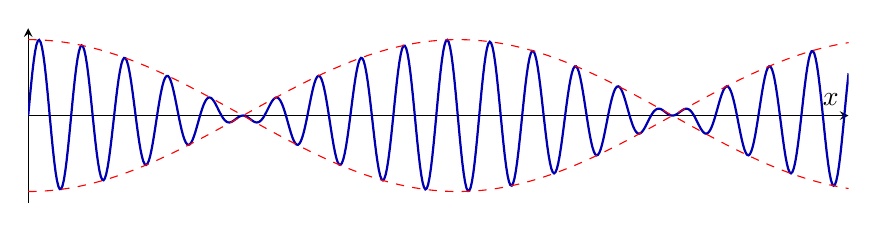
\begin{tikzpicture}
\begin{axis}[width=12cm,height=3.8cm,axis lines=middle,xtick=\empty,ytick=\empty,
  xmin=0,xmax=40,ymin=-2.3,ymax=2.3,samples=600,domain=0:40,xlabel={$x$}]
  \addplot[thick,blue!70!black] {2*sin(deg(3*x))*cos(deg(0.15*x))};
  \addplot[dashed,red] {2*cos(deg(0.15*x))};
  \addplot[dashed,red] {-2*cos(deg(0.15*x))};
\end{axis}
\end{tikzpicture}
\caption{Onda rápida modulada por una envolvente (el coseno).}
\end{figure}

Sumando más ondas senoidales se puede lograr una función que adecuadamente representa a una partícula.

\subsection{Paquete de ondas (grupo de ondas)}
\[
\Psi=\sum_i A_i\sen(k_ix-\omega_it)=\sum_i A_i\,e^{j(k_ix-\omega_it)},\qquad j=\sqrt{-1}
\]
Si el espectro es continuo:
\[
\Psi=\int A(k)\,e^{j(kx-\omega t)}\,dk
\]

\begin{obs}
La igualdad entre la suma de senos y la de exponenciales no es literal (el seno es solo la parte imaginaria de la
exponencial). En mecánica cuántica se toma directamente la forma exponencial compleja como función de onda.
\end{obs}

\textbf{Interpretación de $\Psi$:}
\begin{itemize}
  \item $|\Psi|^2\,dV$: probabilidad de encontrar a la partícula en el volumen $dV$.
  \item $|\Psi|^2$: densidad de probabilidad de encontrarla en un punto.
\end{itemize}

\subsection{Velocidad}
El paquete se desplaza de $t_1$ a $t_2$. En la suma de 2 ondas, la velocidad de grupo es:
\[
v_g=\frac{\Delta\omega/2}{\Delta k/2}=\frac{\Delta\omega}{\Delta k},\qquad \text{velocidad de fase: } v_p=\frac{\omega_0}{k_0}
\]
En nuestro caso (paquete de ondas):
\[
v_g=\frac{d\omega}{dk}\ \ (\text{propagación de la partícula}),\qquad v_p=\frac{\omega}{k}
\]

% ============================================================
\section{Principio de incertidumbre \pags{40--41}}
% ============================================================

\textbf{Heisenberg (1927).}

\subsection{Ejemplo: paquete gaussiano}
Tomamos un paquete de ondas dado por $A(k)=C\,e^{-a^2(k-k_0)^2}$. Halle $\Psi$.

(Espectro discreto: amplitudes $A_1,A_2,A_3$ en $k_1,k_2,k_3$. Espectro continuo: curva $A(k)$.)

\begin{figure}[H]
\centering
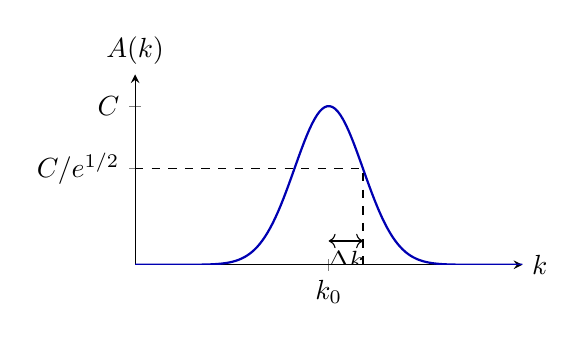
\begin{tikzpicture}
\begin{axis}[width=6.5cm,height=4cm,axis lines=left,xtick={2},xticklabels={$k_0$},ytick={1,0.6065},
  yticklabels={$C$,$C/e^{1/2}$},xmin=0,xmax=4,ymin=0,ymax=1.2,samples=150,domain=0:4,xlabel={$k$},ylabel={$A(k)$},
  every axis x label/.style={at={(ticklabel* cs:1)},anchor=west},
  every axis y label/.style={at={(ticklabel* cs:1)},anchor=south}]
  \addplot[thick,blue!70!black] {exp(-4*(x-2)^2)};
  \draw[dashed] (axis cs:0,0.6065) -- (axis cs:2.354,0.6065) -- (axis cs:2.354,0);
  \draw[<->] (axis cs:2,0.15) -- (axis cs:2.354,0.15) node[midway,below,font=\small]{$\Delta k$};
\end{axis}
\end{tikzpicture}
\hspace{0.6cm}
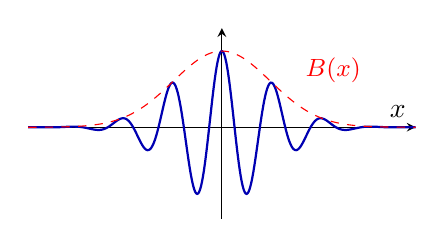
\begin{tikzpicture}
\begin{axis}[width=6.5cm,height=4cm,axis lines=middle,xtick=\empty,ytick=\empty,
  xmin=-4,xmax=4,ymin=-1.2,ymax=1.3,samples=400,domain=-4:4,xlabel={$x$}]
  \addplot[thick,blue!70!black] {exp(-x^2/2)*cos(deg(6*x))};
  \addplot[dashed,red] {exp(-x^2/2)};
  \node[red,font=\small] at (axis cs:2.3,0.75) {$B(x)$};
\end{axis}
\end{tikzpicture}
\caption{Espectro gaussiano $A(k)$ y el paquete $\Psi(x,0)$: onda plana modulada por la amplitud $B(x)$.}
\end{figure}

Despreciamos las amplitudes menores que el máximo$/e^{1/2}$, es decir, $C/e^{1/2}$:
\[
A(k_0+\Delta k)=\frac{C}{e^{1/2}}=C\,e^{-a^2(k_0+\Delta k-k_0)^2}
\ \Rightarrow\
\Delta k=\frac{1}{\sqrt2\,a}
\]
Ahora hallamos $\Psi(x,t)$ cuando $t=0$ $\rightarrow$ $\Psi(x,0)$:
\[
\Psi(x,t)=\int A\,e^{i(kx-\omega t)}\,dk
\]
\[
\Psi(x,0)=\int_{-\infty}^{+\infty}C\,e^{-a^2(k-k_0)^2}\,e^{ikx}\,dk
=\underbrace{C\,\frac{\sqrt\pi}{a}\,e^{-x^2/4a^2}}_{\text{amplitud }B(x)}\ \underbrace{e^{ik_0x}}_{\text{onda plana}}
\]
Con el mismo criterio:
\[
B(0+\Delta x)=\frac{B(0)}{e^{1/2}}
\ \Rightarrow\
C\frac{\sqrt\pi}{a}e^{-(0+\Delta x)^2/4a^2}=\frac{C\frac{\sqrt\pi}{a}e^{-0^2/4a^2}}{e^{1/2}}
\ \Rightarrow\
\frac{(\Delta x)^2}{4a^2}=\frac12
\ \Rightarrow\
\Delta x=\sqrt2\,a
\]
\[
\Delta k\,\Delta x=1=\text{const.}
\]
Con un mejor análisis:
\[
\Delta k\,\Delta x\ge\frac12\qquad
\begin{cases}\Delta k_x\,\Delta x\ge 1/2\\ \Delta k_y\,\Delta y\ge 1/2\\ \Delta k_z\,\Delta z\ge 1/2\end{cases}
\]
Multiplicando por $\hbar$: $\hbar\,\Delta k\,\Delta x\ge\hbar/2$. Pero $p=\hbar k\ \rightarrow\ \Delta p=\hbar\,\Delta k$:
\[
\boxed{\Delta p\,\Delta x\ge\frac{\hbar}{2}}\qquad
\begin{cases}\Delta p_x\,\Delta x\ge\hbar/2\\ \Delta p_y\,\Delta y\ge\hbar/2\\ \Delta p_z\,\Delta z\ge\hbar/2\end{cases}
\]

\begin{obs}
El «mejor análisis» consiste en usar la desviación estándar de $|\Psi|^2$ y $|A(k)|^2$ como medida de anchura (en lugar
del corte en $1/e^{1/2}$); la gaussiana es justo el caso de igualdad $\Delta k\,\Delta x=1/2$.
\end{obs}

\subsection{Otras relaciones de incertidumbre}
\[
\Delta\omega\,\Delta t\ge\frac12
\]
$\Delta t$, $t$: tiempo de vida en un estado. Multiplicando por $\hbar$: $\hbar\,\Delta\omega\,\Delta t\ge\hbar/2$.
Pero $E=h\nu\cdot\frac{2\pi}{2\pi}=\hbar\omega\ \rightarrow\ \Delta E=\hbar\,\Delta\omega$:
\[
\boxed{\Delta E\,\Delta t\ge\frac{\hbar}{2}}
\]
% ============================================================
\section{Mecánica cuántica: postulados y operadores \pags{41--42}}
% ============================================================

\subsection{Postulados de la mecánica cuántica}
\begin{enumerate}
  \item \textbf{La función de onda $\Psi(x,y,z,t)$}
  \begin{itemize}
    \item Representa el estado cuántico de una partícula o sistema.
    \item Su cuadrado del valor absoluto $|\Psi|^2$ da la probabilidad de encontrar la partícula en un lugar del espacio en el tiempo $t$.
    \item Es una función compleja que contiene toda la información del sistema.
  \end{itemize}
  \item \textbf{Variables dinámicas $\rightarrow$ operadores hermíticos}
  \begin{itemize}
    \item Cada magnitud física observable (como posición, momento, energía) se representa mediante un operador matemático.
    \item Estos operadores deben ser hermíticos (autoadjuntos) para asegurar que sus valores propios (mediciones posibles) sean reales.
  \end{itemize}
  \item \textbf{Ecuación de valores propios:} $\hat A\Psi=A\Psi$
  \begin{itemize}
    \item $\hat A$: operador asociado a una magnitud física.
    \item $A$: valor propio.
    \item $\Psi$: función propia asociada a ese valor.
  \end{itemize}
  \item \textbf{Valor esperado de esa magnitud:}
  \[
  \langle A\rangle=\int\Psi^*\,\hat A\,\Psi\,dV
  \]
  \begin{itemize}
    \item $\langle A\rangle$: valor promedio que esperamos obtener.
    \item $\Psi^*$: conjugado complejo de la función de onda.
    \item La integral se hace sobre todo el espacio.
  \end{itemize}
  \item \textbf{Ecuación de Schrödinger}
  \[
  i\hbar\,\frac{\partial\Psi}{\partial t}=\hat H\Psi
  \]
  \begin{itemize}
    \item $i$: unidad imaginaria ($i=\sqrt{-1}$).
    \item $\hbar$: constante de Planck reducida, $\hbar=h/2\pi$.
    \item $\Psi$: función de onda que representa el estado del sistema.
    \item $\partial\Psi/\partial t$: cómo cambia la función de onda con el tiempo.
    \item $\hat H$: hamiltoniano, es decir, el operador de energía total del sistema (energía cinética $+$ potencial).
  \end{itemize}
\end{enumerate}

Nota al margen del cuaderno (promedio de una función): $\displaystyle\langle f\rangle=\frac{\int f\,dt}{\int dt}$.

\textbf{$\Psi$ no puede ser, por ejemplo, $e^x$} (diverge), ni una función con saltos (discontinua):
\begin{figure}[H]
\centering
\begin{tikzpicture}[scale=0.8]
  \draw[->] (-1.5,0) -- (2.2,0) node[right]{$x$};
  \draw[->] (0,-0.3) -- (0,3) node[above]{$\Psi$};
  \draw[thick,red!70!black,domain=-1.5:1.1,samples=50] plot (\x,{exp(\x)});
  \node[font=\small] at (0.3,-0.8) {$e^x$: diverge};
  \begin{scope}[xshift=5.5cm]
  \draw[->] (-1.5,0) -- (2.2,0) node[right]{$x$};
  \draw[->] (0,-0.3) -- (0,3) node[above]{$\Psi$};
  \draw[thick,red!70!black] (-1.4,0.6) -- (0.5,1.2); \draw[thick,red!70!black] (0.5,2.2) -- (2,2.5);
  \draw[dotted] (0.5,1.2) -- (0.5,2.2);
  \node[font=\small] at (0.3,-0.8) {discontinua};
  \end{scope}
\end{tikzpicture}
\caption{Funciones que no pueden ser una función de onda.}
\end{figure}

\begin{obs}
Las condiciones implícitas son que $\Psi$ sea finita (normalizable), continua y de un solo valor; y, donde el potencial
es finito, también $d\Psi/dx$ continua.
\end{obs}

\subsection{Operadores}
\[
\vec\nabla=\frac{\partial}{\partial x}\ii+\frac{\partial}{\partial y}\jj+\frac{\partial}{\partial z}\kk,\qquad
\vec\nabla f=\frac{\partial f}{\partial x}\ii+\frac{\partial f}{\partial y}\jj+\frac{\partial f}{\partial z}\kk
\]

\begin{center}
\begin{tabular}{lcc}
\toprule
Operador & ¿Lineal? & ¿Hermítico?\\
\midrule
$\hat A=\sqrt{\ }$ & No & ---\\
$\hat B=\partial/\partial x$ & Sí & No\\
$\hat C=i\,\partial/\partial x$ & Sí & Sí\\
\bottomrule
\end{tabular}
\end{center}

\textbf{Lineal:} $\hat D(f_1+f_2)=\hat Df_1+\hat Df_2$ \ y \ $\hat D(cf)=c\,\hat Df$.

\textbf{Hermítico:} sus valores propios son reales $\therefore$ son adecuados para representar una magnitud física.

\subsection{Algunos operadores}
\[
\hat H=\hat T+\hat U\quad(\hat T:\ \text{energía cinética},\ \hat U:\ \text{energía potencial}),\qquad
\hat T=\frac{\hat p^2}{2m},\qquad \hat U=U
\]
\[
\hat p=-i\hbar\vec\nabla\ \rightarrow\ \hat p^2=(-i\hbar\vec\nabla)^2=-\hbar^2\Delta
\]
Ej.: en el eje $x$:
\[
\hat p^2=-\hbar^2\frac{\partial^2}{\partial x^2},\qquad
\hat T=-\frac{\hbar^2}{2m}\frac{\partial^2}{\partial x^2},\qquad
\hat L=\hat r\times\hat p,\quad \hat r=\vec r
\]

% ============================================================
\section{Partícula libre \pags{42--43}}
% ============================================================

Partícula libre: $U=0$. Resolvamos la ecuación de Schrödinger:
\[
i\hbar\frac{\partial\Psi}{\partial t}=(\hat T+\hat U)\Psi=(\hat T+U)\Psi
\]
En 1 dimensión (eje $x$): $\Psi=\Psi(x,t)$, \ $\hat T=-\dfrac{\hbar^2}{2m}\dfrac{\partial^2}{\partial x^2}$:
\[
i\hbar\frac{\partial\Psi}{\partial t}=\left(-\frac{\hbar^2}{2m}\frac{\partial^2}{\partial x^2}+0\right)\Psi
\]
\textbf{Separación de variables:} $\Psi(x,t)=\varphi(x)\cdot\gamma(t)$
\[
i\hbar\,\varphi\frac{\partial\gamma}{\partial t}=-\frac{\hbar^2}{2m}\gamma\frac{\partial^2\varphi}{\partial x^2}
\quad\xrightarrow{\ \div\,\varphi\gamma\ }\quad
\underbrace{\frac{i\hbar\,\partial\gamma/\partial t}{\gamma}}_{\text{de }t}
=\underbrace{\frac{-\frac{\hbar^2}{2m}\,\partial^2\varphi/\partial x^2}{\varphi}}_{\text{de }x}=\text{const}=E
\]
Forma general de la solución: $f=A\,e^{r_1x}+B\,e^{r_2x}$.

Volviendo al problema:
\[
\frac{\hbar^2}{2m}\frac{d^2\varphi}{dx^2}+E\varphi=0
\]
Solución $e^{\rho x}$:
\[
\frac{\hbar^2}{2m}\rho^2+E=0\ \Rightarrow\ \rho=\pm\frac{i}{\hbar}\sqrt{2mE}
\ \Rightarrow\
\varphi=A\,e^{\frac{i}{\hbar}\sqrt{2mE}\,x}+B\,e^{-\frac{i}{\hbar}\sqrt{2mE}\,x}
\]
Hacemos:
\[
k=\frac{\sqrt{2mE}}{\hbar},\qquad \omega=\frac{E}{\hbar}
\]
\[
\Psi(x,t)=\varphi\gamma=C_1\,e^{i(kx-\omega t)}+C_2\,e^{-i(kx-\omega t)}
\]
Superposición de 2 ondas planas en direcciones opuestas.

\begin{obs}
El segundo término debería ser $C_2\,e^{-i(kx+\omega t)}$, porque $\gamma(t)=e^{-i\omega t}$ multiplica a ambos términos de
$\varphi$. Tal como está escrito, el segundo término tendría energía $-E$. La conclusión (dos ondas en direcciones
opuestas) no cambia.
\end{obs}

Supongamos que se conoce que la partícula viaja hacia la derecha: $C_2=0$.
\[
\Psi=C_1\,e^{i(kx-\omega t)}=e^{\frac{i}{\hbar}(px-Et)}
\]
Onda plana infinita: $\Delta E=0$, $\Delta p=0$, $\Delta x=\infty$ (de acuerdo con el principio de incertidumbre).

% ============================================================
\section{Ecuación de Schrödinger independiente del tiempo \pags{43}}
% ============================================================

Casos estacionarios: $U(x,y,z,t)=U(x,y,z)$.
\[
i\hbar\frac{\partial\Psi}{\partial t}=(\hat T+U)\Psi=\left(-\frac{\hbar^2}{2m}\nabla^2+U\right)\Psi
\]
Separación de variables: $\Psi(x,t)=\varphi(x)\cdot\gamma(t)$
\[
i\hbar\frac{\partial}{\partial t}(\varphi\gamma)=\left(-\frac{\hbar^2}{2m}\nabla^2+U\right)(\varphi\gamma)
\ \Rightarrow\
i\hbar\,\varphi\frac{\partial\gamma}{\partial t}=\gamma\underbrace{\left(-\frac{\hbar^2}{2m}\nabla^2+U\right)}_{\hat H}\varphi
\]
Dividiendo entre $(\varphi\gamma)$:
\[
\underbrace{\frac{i\hbar\,\partial\gamma/\partial t}{\gamma}}_{\text{de }t}=\underbrace{\frac{\hat H\varphi}{\varphi}}_{\text{de }x,y,z}=\text{const}=E
\qquad
\begin{cases} i\hbar\,\dfrac{\partial\gamma}{\partial t}=E\gamma & (1)\\[3mm] \hat H\varphi=E\varphi & (2)\end{cases}
\]
(2) es la \textbf{ecuación de Schrödinger independiente del tiempo}.

\begin{obs}
La ecuación (1) se resuelve una sola vez para todos los problemas: $\gamma(t)=e^{-iEt/\hbar}$. Por eso en los problemas
siguientes basta resolver (2).
\end{obs}

% ============================================================
\section{Pozo de potencial infinito \pags{43--44}}
% ============================================================

(Analogía en el cuaderno: un pozo en el terreno, donde $U=mgh$.)
\[
U=\begin{cases}0, & 0\le x\le a\\ \infty, & \text{en el resto}\end{cases}
\]

\textbf{Intervalo $0\le x\le a$:} $U=0$, $\hat H\varphi=E\varphi$. En 1 dimensión:
\[
\left(-\frac{\hbar^2}{2m}\frac{\partial^2}{\partial x^2}+U\right)\varphi=E\varphi
\ \rightarrow\
\left(-\frac{\hbar^2}{2m}\frac{\partial^2}{\partial x^2}+0\right)\varphi=E\varphi
\]
Ya hemos resuelto:
\[
\varphi=A\,e^{ikx}+B\,e^{-ikx},\qquad k=\frac1\hbar\sqrt{2mE}
\]
\textbf{Intervalo restante:} $U=\infty$ $\rightarrow$ la partícula no podrá estar ahí: $|\varphi|^2=0$, o sea $\varphi=0$.

\subsection{Condición de continuidad}
Frontera $x=0$: $\varphi(0^-)=\varphi(0^+)$
\[
0=A\,e^{ik(0)}+B\,e^{-ik(0)}\ \Rightarrow\ B=-A\ \Rightarrow\ \varphi=2iA\sen kx
\]
Frontera $x=a$: $\varphi(a^-)=\varphi(a^+)$
\[
2iA\sen ka=0\ \Rightarrow\ k=\frac{n\pi}{a},\quad n=1,2,3,4,\ldots
\ \Rightarrow\
\varphi=2iA\sen\!\left(\frac{n\pi}{a}x\right)
\]

\subsection{Energía}
Teníamos $k=\frac1\hbar\sqrt{2mE}$:
\[
\frac{n\pi}{a}=\frac1\hbar\sqrt{2mE}\ \Rightarrow\ \boxed{E=\frac{\hbar^2\pi^2}{2ma^2}\,n^2},\qquad n=1,2,3,\ldots
\]

\begin{figure}[H]
\centering
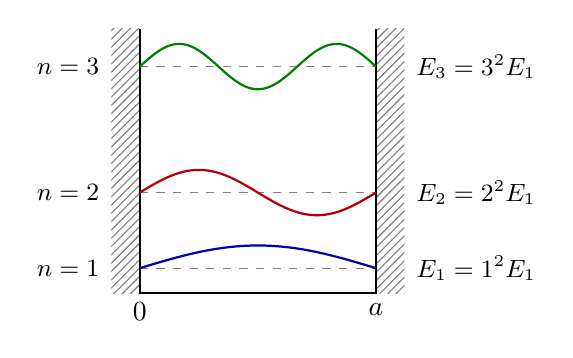
\begin{tikzpicture}[xscale=3,yscale=0.32]
  \fill[pattern=north east lines,pattern color=gray] (-0.12,0) rectangle (0,10.5);
  \fill[pattern=north east lines,pattern color=gray] (1,0) rectangle (1.12,10.5);
  \draw[thick] (0,10.5) -- (0,0) -- (1,0) -- (1,10.5);
  \node[below] at (0,0) {$0$}; \node[below] at (1,0) {$a$};
  \foreach \n/\c in {1/blue!70!black,2/red!70!black,3/green!50!black}{
    \pgfmathsetmacro{\E}{\n*\n}
    \draw[dashed,gray] (0,\E) -- (1,\E);
    \draw[thick,\c,domain=0:1,samples=80] plot (\x,{\E+0.9*sin(deg(\n*pi*\x))});
    \node[right,font=\small] at (1.13,\E) {$E_\n=\n^2E_1$};
  }
  \node[left,font=\small] at (-0.13,1) {$n=1$};
  \node[left,font=\small] at (-0.13,4) {$n=2$};
  \node[left,font=\small] at (-0.13,9) {$n=3$};
\end{tikzpicture}
\caption{Niveles de energía y funciones de onda del pozo infinito, con $E_1=\hbar^2\pi^2/(2ma^2)$.}
\end{figure}

\subsection{Condición de normalización}
\[
\int_{-\infty}^{+\infty}|\varphi|^2\,dx=1,\qquad |\varphi|^2=\varphi^*\varphi
\]
\[
\int_{-\infty}^{+\infty}=\int_{-\infty}^{0}+\int_0^a+\int_a^{+\infty}
=\int_0^a\left(-2iA\sen\frac{n\pi}{a}x\right)\left(2iA\sen\frac{n\pi}{a}x\right)dx=1
\]
\[
A=\frac{1}{\sqrt{2a}}\ \Rightarrow\ \boxed{\varphi=i\sqrt{\frac2a}\,\sen\!\left(\frac{n\pi}{a}x\right)}
\]

\begin{obs}
El factor $i$ es una fase global y no tiene efecto físico; muchos libros escriben simplemente
$\varphi=\sqrt{2/a}\,\sen(n\pi x/a)$. También: $n=0$ se descarta porque da $\varphi=0$ (no hay partícula).
\end{obs}

% ============================================================
\section{Potencial escalón \pags{44--46}}
% ============================================================

\[
U=\begin{cases}0, & x<0\\ U_0, & x\ge0\end{cases}\qquad\qquad \hat H\varphi=E\varphi
\]

\textbf{Intervalo $x<0$:} $U=0$
\[
\left(-\frac{\hbar^2}{2m}\frac{d^2}{dx^2}+0\right)\varphi=E\varphi
\ \Rightarrow\
\varphi=A\,e^{ik_1x}+B\,e^{-ik_1x},\qquad k_1=\frac1\hbar\sqrt{2mE}
\]
\textbf{Intervalo $x\ge0$:} $U=U_0$
\[
\left(-\frac{\hbar^2}{2m}\frac{d^2}{dx^2}+U_0\right)\varphi=E\varphi
\ \Rightarrow\
\frac{\hbar^2}{2m}\frac{d^2\varphi}{dx^2}+(E-U_0)\varphi=0
\]
Es de la forma $Af''+Bf'+Cf=0$. Solución: $e^{\rho x}$. Reemplazar:
\[
\frac{\hbar^2}{2m}\rho^2e^{\rho x}+(E-U_0)e^{\rho x}=0
\ \Rightarrow\
\frac{\hbar^2}{2m}\rho^2+(E-U_0)=0
\ \Rightarrow\
\rho=\pm\frac1\hbar\sqrt{-2m(E-U_0)}
\]

\subsection{1.\textsuperscript{er} caso: $E>U_0$}
\[
\rho=\pm\frac{i}{\hbar}\sqrt{2m(E-U_0)}=\pm ik_2,\qquad k_2=\frac1\hbar\sqrt{2m(E-U_0)}
\]
\[
\varphi=C\,e^{ik_2x}+D\,e^{-ik_2x}
\]
$k_2<k_1\ \rightarrow\ \lambda_2>\lambda_1$: la onda sigue oscilando a la derecha, pero con mayor longitud de onda.

\subsection{2.\textsuperscript{do} caso: $E\le U_0$}
\[
\rho=\pm\frac1\hbar\sqrt{2m(U_0-E)}\ \ (\text{real})=\pm\sigma,\qquad \sigma=\frac1\hbar\sqrt{2m(U_0-E)}
\]
\[
\varphi=C\,e^{\sigma x}+D\,e^{-\sigma x}
\]
El término $e^{\sigma x}$ crece sin límite, así que hacemos $C=0$:
\[
\varphi=D\,e^{-\sigma x}
\]
En el 2.\textsuperscript{do} caso suponemos que una partícula se mueve a la derecha desde $-\infty$.

\begin{figure}[H]
\centering
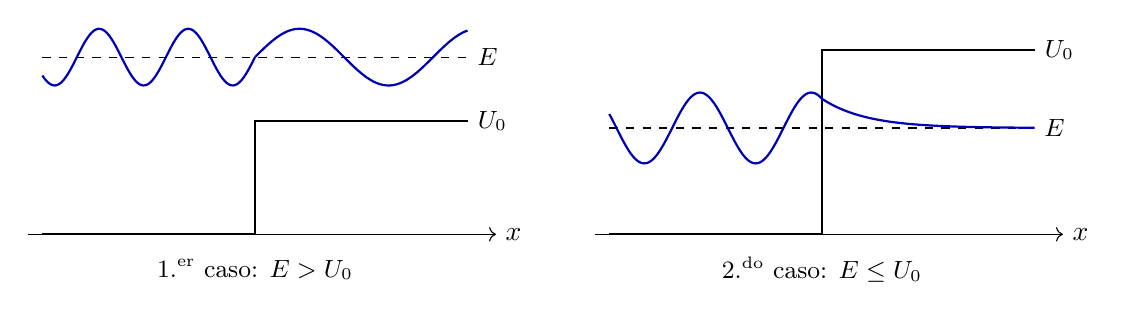
\begin{tikzpicture}[scale=0.9]
  \begin{scope}
  \draw[->] (-3.2,0) -- (3.4,0) node[right]{$x$};
  \draw[thick] (-3,0) -- (0,0) -- (0,1.6) -- (3,1.6) node[right,font=\small]{$U_0$};
  \draw[dashed] (-3,2.5) -- (3,2.5) node[right,font=\small]{$E$};
  \draw[blue!70!black,thick,domain=-3:0,samples=100] plot (\x,{2.5+0.4*sin(deg(5*\x))});
  \draw[blue!70!black,thick,domain=0:3,samples=100] plot (\x,{2.5+0.4*sin(deg(2.5*\x))});
  \node[font=\small] at (0,-0.5) {1.\textsuperscript{er} caso: $E>U_0$};
  \end{scope}
  \begin{scope}[xshift=8cm]
  \draw[->] (-3.2,0) -- (3.4,0) node[right]{$x$};
  \draw[thick] (-3,0) -- (0,0) -- (0,2.6) -- (3,2.6) node[right,font=\small]{$U_0$};
  \draw[dashed] (-3,1.5) -- (3,1.5) node[right,font=\small]{$E$};
  \draw[blue!70!black,thick,domain=-3:0,samples=100] plot (\x,{1.5+0.5*cos(deg(4*\x+0.6))});
  \draw[blue!70!black,thick,domain=0:3,samples=60] plot (\x,{1.5+0.5*cos(deg(0.6))*exp(-1.6*\x)});
  \node[font=\small] at (0,-0.5) {2.\textsuperscript{do} caso: $E\le U_0$};
  \end{scope}
\end{tikzpicture}
\caption{Potencial escalón: en el 2.\textsuperscript{do} caso $\varphi$ decae exponencialmente dentro del escalón.}
\end{figure}

Para $x>0$, $|\varphi|^2$ \textbf{no es despreciable}: la partícula penetra en la región clásicamente prohibida.

\subsection{Ejemplo: coeficientes de reflexión y transmisión ($E>U_0$)}
Para una partícula que se mueve desde $-\infty$ hacia la derecha en el eje $x$ con $E>U_0$, halle el coeficiente de
reflexión y de transmisión.

\textbf{Sol.:} $v|\varphi|^2\approx\dfrac{dx}{dt}|\varphi|^2\ \rightarrow$ corriente de probabilidad.
\[
\varphi_I=A\,e^{ik_1x}+B\,e^{-ik_1x}\ \ (\text{región I},\ x<0),\qquad
\varphi_{II}=C\,e^{ik_2x}+D\,e^{-ik_2x}\ \ (\text{región II},\ x>0)
\]
La onda transmitida ya no se refleja $\rightarrow$ $D=0$.
\begin{itemize}
  \item $C\,e^{ik_2x}=\varphi_t$ $\rightarrow$ onda transmitida
  \item $B\,e^{-ik_1x}=\varphi_r$ $\rightarrow$ onda reflejada
  \item $A\,e^{ik_1x}=\varphi_i$ $\rightarrow$ onda incidente
\end{itemize}
\[
R=\frac{v_r|\varphi_r|^2}{v_i|\varphi_i|^2}=\frac{v_I\,Be^{-ik_1x}B^*e^{ik_1x}}{v_I\,Ae^{ik_1x}A^*e^{-ik_1x}}=\frac{|B|^2}{|A|^2},
\qquad
T=\frac{v_t|\varphi_t|^2}{v_i|\varphi_i|^2}=\frac{v_{II}|C|^2}{v_I|A|^2}
\]
Con $p=mv=\hbar k$: \ $mv_{II}=\hbar k_2$, \ $mv_I=\hbar k_1$ \ (y $\varphi^*\varphi=|\varphi|^2$, $B^*B=|B|^2$).

\textbf{Hallemos $A$, $B$, $C$.} De la condición de continuidad: $\varphi(0^-)=\varphi(0^+)$ y $\varphi'(0^-)=\varphi'(0^+)$.
\[
Ae^0+Be^0=Ce^0\ \Rightarrow\ A+B=C\qquad(\alpha)
\]
Derivamos: $ik_1Ae^{ik_1x}-ik_1Be^{-ik_1x}\ \big|\ ik_2Ce^{ik_2x}$
\[
ik_1A-ik_1B=ik_2C\qquad(\beta)
\]
De $(\alpha)$ y $(\beta)$:
\[
2ik_1A=i(k_1+k_2)C\ \Rightarrow\ C=\frac{2k_1A}{k_1+k_2},\qquad
B=\frac{2k_1A}{k_1+k_2}-A=\frac{k_1-k_2}{k_1+k_2}A
\]
\[
\boxed{R=\left(\frac{k_1-k_2}{k_1+k_2}\right)^2,\qquad T=\frac{k_2}{k_1}\cdot\frac{4k_1^2}{(k_1+k_2)^2}=\frac{4k_1k_2}{(k_1+k_2)^2}}
\]

\begin{obs}
Comprobación rápida: $R+T=\dfrac{(k_1-k_2)^2+4k_1k_2}{(k_1+k_2)^2}=1$. Aunque $E>U_0$, hay reflexión ($R\neq0$), algo
imposible en física clásica.
\end{obs}

% ============================================================
\section{Efecto túnel \pags{46}}
% ============================================================

Barrera de altura $U_0$ entre $x=0$ y $x=a$; una partícula con $E<U_0$ llega desde la izquierda.
(El cuaderno solo deja el esquema de la barrera, sin desarrollo.)

\begin{figure}[H]
\centering
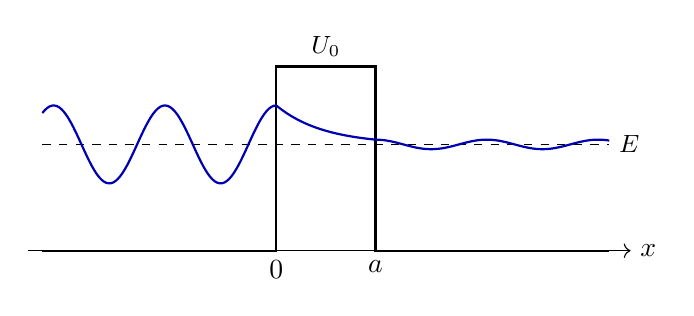
\begin{tikzpicture}[scale=0.9]
  \draw[->] (-3.5,0) -- (5,0) node[right]{$x$};
  \draw[thick] (-3.3,0) -- (0,0) -- (0,2.6) -- (1.4,2.6) -- (1.4,0) -- (4.7,0);
  \node[below] at (0,0) {$0$}; \node[below] at (1.4,0) {$a$};
  \node[above,font=\small] at (0.7,2.6) {$U_0$};
  \draw[dashed] (-3.3,1.5) -- (4.7,1.5) node[right,font=\small]{$E$};
  \draw[blue!70!black,thick,domain=-3.3:0,samples=100] plot (\x,{1.5+0.55*cos(deg(4*\x))});
  \draw[blue!70!black,thick,domain=0:1.4,samples=40] plot (\x,{1.5+0.55*exp(-1.5*\x)});
  \draw[blue!70!black,thick,domain=1.4:4.7,samples=100] plot (\x,{1.5+0.55*exp(-2.1)*cos(deg(4*(\x-1.4)))});
\end{tikzpicture}
\caption{Barrera de potencial: la onda decae dentro de la barrera y sale con amplitud menor.}
\end{figure}

\begin{obs}
Por lo visto en el 2.\textsuperscript{do} caso del escalón, dentro de la barrera $\varphi$ decae como $e^{-\sigma x}$ pero no se
anula; si la barrera es delgada, sale una onda transmitida. Para una barrera ancha ($\sigma a\gg1$),
$T\approx e^{-2\sigma a}$, con $\sigma=\sqrt{2m(U_0-E)}/\hbar$.
\end{obs}
% ============================================================
\section{Caja de potencial tridimensional \pags{46--48}}
% ============================================================

\[
U=\begin{cases}0, & 0\le x\le a,\ 0\le y\le b,\ 0\le z\le c\\ \infty, & \text{en el resto}\end{cases}
\]
\[
\hat H\varphi=E\varphi:\qquad
\left[-\frac{\hbar^2}{2m}\left(\frac{\partial^2}{\partial x^2}+\frac{\partial^2}{\partial y^2}+\frac{\partial^2}{\partial z^2}\right)+U\right]\varphi=E\varphi
\]
\textbf{Separación de variables:} $\varphi(x,y,z)=\varphi_1(x)\cdot\varphi_2(y)\cdot\varphi_3(z)$. Dentro de la caja, $U=0$:
\[
-\frac{\hbar^2}{2m}\left(\varphi_2\varphi_3\frac{\partial^2\varphi_1}{\partial x^2}+\varphi_1\varphi_3\frac{\partial^2\varphi_2}{\partial y^2}+\varphi_1\varphi_2\frac{\partial^2\varphi_3}{\partial z^2}\right)=E\,\varphi_1\varphi_2\varphi_3
\]
Dividimos entre $\varphi_1\varphi_2\varphi_3$:
\[
\underbrace{\frac{\partial^2\varphi_1/\partial x^2}{\varphi_1}}_{\text{de }x}+\underbrace{\frac{\partial^2\varphi_2/\partial y^2}{\varphi_2}}_{\text{de }y}+\underbrace{\frac{\partial^2\varphi_3/\partial z^2}{\varphi_3}}_{\text{de }z}
=-\frac{2mE}{\hbar^2}=-\alpha^2=-\alpha_1^2-\alpha_2^2-\alpha_3^2
\]
(Idea del margen: si una función de $t$ es igual a una función de $x$, ambas son una constante; si la suma de funciones
de variables distintas es constante, cada una es constante.)
\[
\frac{\partial^2\varphi_1}{\partial x^2}=-\alpha_1^2\varphi_1\ (1),\qquad
\frac{\partial^2\varphi_2}{\partial y^2}=-\alpha_2^2\varphi_2\ (2),\qquad
\frac{\partial^2\varphi_3}{\partial z^2}=-\alpha_3^2\varphi_3\ (3),\qquad
\alpha^2=\frac{2mE}{\hbar^2}=\alpha_1^2+\alpha_2^2+\alpha_3^2
\]
\textbf{Resolvemos (1):} solución $e^{\rho x}$. Reemplazamos: $\rho^2e^{\rho x}=-\alpha_1^2e^{\rho x}\ \rightarrow\ \rho=\pm i\alpha_1$.
\[
\varphi_1=A_1e^{i\alpha_1x}+B_1e^{-i\alpha_1x}
\]
Cambiamos $k_x=\alpha_1$, $k_y=\alpha_2$, $k_z=\alpha_3$:
\[
\varphi_1=A_1e^{ik_xx}+B_1e^{-ik_xx},\quad \varphi_2=A_2e^{ik_yy}+B_2e^{-ik_yy},\quad \varphi_3=A_3e^{ik_zz}+B_3e^{-ik_zz}
\]
Fuera de la caja: $\varphi=0$.

\subsection{Continuidad}
En $x$, fronteras $x=0$ y $x=a$. En $x=0$: $\varphi(0^-)=\varphi(0^+)$:
\[
0=(A_1e^0+B_1e^0)\varphi_2\varphi_3\ \Rightarrow\ B_1=-A_1\ \Rightarrow\ \varphi_1=A_1(e^{ik_xx}-e^{-ik_xx})=2iA_1\sen(k_xx)
\]
En analogía: en $y$ ($y=0$) $\rightarrow$ $\varphi_2=2iA_2\sen(k_yy)$; en $z$ ($z=0$) $\rightarrow$ $\varphi_3=2iA_3\sen(k_zz)$.
\[
\Rightarrow\ \varphi=C\sen(k_xx)\sen(k_yy)\sen(k_zz)
\]
Continuidad en $x=a$: $\varphi(a^-)=\varphi(a^+)\ \rightarrow\ C\sen(k_xa)\sen(k_yy)\sen(k_zz)=0$:
\[
k_x=n_1\frac{\pi}{a},\qquad k_y=n_2\frac{\pi}{b},\qquad k_z=n_3\frac{\pi}{c},\qquad n_1,n_2,n_3=1,2,3,\ldots
\]

\subsection{Energía}
Habíamos escrito:
\[
\frac{2mE}{\hbar^2}=\alpha^2=\alpha_1^2+\alpha_2^2+\alpha_3^2=k_x^2+k_y^2+k_z^2
\ \Rightarrow\
E=\frac{\hbar^2}{2m}(k_x^2+k_y^2+k_z^2)=\frac{\hbar^2k^2}{2m}
\]
\[
\boxed{E=\frac{\hbar^2}{2m}\left[\frac{n_1^2\pi^2}{a^2}+\frac{n_2^2\pi^2}{b^2}+\frac{n_3^2\pi^2}{c^2}\right]}
\]

\subsection{Ejemplo: caja cúbica de lado $L$}
Halle los niveles de energía de una partícula en una caja cúbica de lado $L$. Solución: $a=b=c=L$.
\[
\varphi=C\sen\!\left(\frac{n_1\pi}{L}x\right)\sen\!\left(\frac{n_2\pi}{L}y\right)\sen\!\left(\frac{n_3\pi}{L}z\right),\qquad
E=\frac{\hbar^2\pi^2}{2mL^2}\,(n_1^2+n_2^2+n_3^2)
\]

\begin{center}
\begin{tabular}{llc}
\toprule
Nivel & $(n_1,n_2,n_3)$ anotados & $E$ en unidades de $\hbar^2\pi^2/(2mL^2)$\\
\midrule
1.\textsuperscript{er} & (1,1,1) & 3\\
2.\textsuperscript{do} & (2,1,1), (1,2,1), (1,1,2) & 6\\
3.\textsuperscript{er} & (2,2,1), (2,1,2), (1,2,2) & 9\\
4.\textsuperscript{to} & (3,1,1), (1,3,1), (1,1,3) & 11\\
5.\textsuperscript{to} & (2,2,2) & 12\\
6.\textsuperscript{to} & (1,3,2), (2,1,3), (3,2,1) & 14\\
\bottomrule
\end{tabular}
\end{center}

Estados del 2.\textsuperscript{do} nivel (estados degenerados):
\[
\begin{gathered}
\varphi_{211}=C\sen\tfrac{2\pi}{L}x\,\sen\tfrac{\pi}{L}y\,\sen\tfrac{\pi}{L}z\\
\varphi_{121}=C\sen\tfrac{\pi}{L}x\,\sen\tfrac{2\pi}{L}y\,\sen\tfrac{\pi}{L}z\\
\varphi_{112}=C\sen\tfrac{\pi}{L}x\,\sen\tfrac{\pi}{L}y\,\sen\tfrac{2\pi}{L}z
\end{gathered}
\]

\textbf{Estados degenerados:} diferentes estados que corresponden a un mismo valor de energía o nivel.

\textbf{Orden de degeneración:} número total de estados en un nivel.

\begin{obs}
En el 5.\textsuperscript{to} nivel el cuaderno repite tres columnas de (2,2,2), pero es un solo estado (orden de degeneración 1).
En el 6.\textsuperscript{to} nivel faltan permutaciones: (1,2,3) y sus permutaciones dan orden de degeneración \textbf{6}, no 3.
Faltan (1,2,3), (2,3,1) y (3,1,2).
\end{obs}

\subsection{¿Cómo se representa un estado?}
\begin{itemize}
  \item La función de onda determina un estado.
  \item Los números cuánticos determinan un estado.
  \item $k_x$, $k_y$ y $k_z$ determinan un estado.
\end{itemize}
\textbf{Espacio-$k$:} cada punto $(k_x,k_y,k_z)$ es un estado, con $\vec k=k_x\ii+k_y\jj+k_z\kk$. Como $E=\hbar^2k^2/2m$,
la superficie isoenergética es una \textbf{esfera}.

% ============================================================
\section{Oscilador armónico \pags{48--50}}
% ============================================================

\[
F=-kx,\qquad \omega=\sqrt{\frac km},\qquad U=\frac{kx^2}{2};\qquad -\infty<x<+\infty
\]
\[
\hat H\varphi=E\varphi:\qquad \left(-\frac{\hbar^2}{2m}\frac{d^2}{dx^2}+\frac{kx^2}{2}\right)\varphi=E\varphi
\ \Rightarrow\
\frac{d^2\varphi}{dx^2}+\left(\frac{2mE}{\hbar^2}-\frac{mkx^2}{\hbar^2}\right)\varphi=0
\]
Hacemos $\alpha^2=\dfrac{mk}{\hbar^2}$ y $\alpha\beta=\dfrac{2mE}{\hbar^2}$:
\[
\frac{d^2\varphi}{dx^2}+(\alpha\beta-\alpha^2x^2)\varphi=0\qquad(1)
\]
\textbf{Cambio de variable:} $\xi=\sqrt\alpha\,x$
\[
\frac{d\varphi}{dx}=\frac{d\varphi}{d\xi}\cdot\frac{d\xi}{dx}=\sqrt\alpha\,\frac{d\varphi}{d\xi},\qquad
\frac{d^2\varphi}{dx^2}=\frac{d}{d\xi}\left(\sqrt\alpha\frac{d\varphi}{d\xi}\right)\frac{d\xi}{dx}=\alpha\frac{d^2\varphi}{d\xi^2}
\]
Reemplazando:
\[
\alpha\frac{d^2\varphi}{d\xi^2}+(\alpha\beta-\alpha\xi^2)\varphi=0\ \Rightarrow\ \frac{d^2\varphi}{d\xi^2}+(\beta-\xi^2)\varphi=0\qquad(2)
\]
Solución de la forma $\varphi=\varphi_\infty\cdot\Phi$, donde $\varphi_\infty$ es la solución asintótica (para $\xi\to\infty$).

\textbf{Solución asintótica:} $\xi\to\infty\ \rightarrow\ \dfrac{d^2\varphi}{d\xi^2}-\xi^2\varphi=0$. Solución $e^{\sigma\xi^2}$; se obtiene
$\sigma=\tfrac12$ (descartada) y $\sigma=-\tfrac12$ (función finita):
\[
\varphi_\infty=A\,e^{-\frac12\xi^2}\ \Rightarrow\ \varphi=A\,e^{-\frac12\xi^2}\,\Phi
\]
Reemplazando en (2) y reordenando (\textbf{ecuación diferencial de Hermite}):
\[
\frac{d^2\Phi}{d\xi^2}-2\xi\frac{d\Phi}{d\xi}+(\beta-1)\Phi=0\qquad(3)
\]
\textbf{Solución: serie de potencias}
\[
\Phi=C_0+C_1\xi+C_2\xi^2+C_3\xi^3+\cdots=\sum_{m=0}^{\infty}C_m\xi^m
\]
Reemplazando en (3):
\[
C_{m+2}=\frac{2m+1-\beta}{(m+1)(m+2)}\,C_m
\]
Si conocemos $C_0$ y $C_1$, se pueden encontrar los demás $C_m$. Por otro lado, la función debe ser finita $\rightarrow$ la
serie debe cortarse (debe converger):
\[
\frac{2m+1-\beta}{(m+1)(m+2)}\le0,\qquad 2m+1-\beta=0\ \Rightarrow\ m_{\text{máx}}=\frac{\beta+1}{2}
\]
Llamamos $n=m_{\text{máx}}=\dfrac{\beta-1}{2}$ \ ($\beta=2n+1$) $\rightarrow$ $C_{n+1}=C_{n+2}=C_{n+3}=\cdots=0$.

\begin{obs}
De $2m+1-\beta=0$ sale $m_{\text{máx}}=(\beta-1)/2$; el «$\beta+1$» de la primera línea es un desliz, que se corrige en la
línea siguiente.
\end{obs}

Además, $C_n=2^n$. Conocemos $C_n=2^n$ y $C_{n+1}=0$, y bajamos con la recurrencia invertida:
\[
C_m=\frac{(m+1)(m+2)}{2m+1-\beta}\,C_{m+2}
\]

\subsection{Energía}
\[
\alpha^2=\frac{mk}{\hbar^2},\ \ \alpha\beta=\frac{2mE}{\hbar^2}
\ \Rightarrow\
\beta=\frac{2mE/\hbar^2}{\sqrt{mk}/\hbar}=\frac{2E}{\hbar\sqrt{k/m}}
\]
\[
\Rightarrow\
E=\frac{\hbar\omega}{2}\beta,\ \ \beta=2n+1
\ \Rightarrow\
\boxed{E=\left(\frac{2n+1}{2}\right)\hbar\omega}
\]

\begin{center}
\renewcommand{\arraystretch}{1.3}
\footnotesize
\setlength{\tabcolsep}{4pt}
\begin{tabular}{clccc}
\toprule
$n$ & Coeficientes & $\Phi(\xi)$ & $\varphi(\xi)$ & $E$\\
\midrule
0 & $C_0=2^0=1$;\ $C_1=C_2=\cdots=0$ & $1$ & $Ae^{-\xi^2/2}\cdot1$ & $\tfrac12\hbar\omega$\\
1 & $C_1=2$;\ $C_2=C_3=\cdots=0$;\ $C_0=[\ ]\cdot C_2=0$ & $2\xi$ & $Ae^{-\xi^2/2}\cdot2\xi$ & $\tfrac32\hbar\omega$\\
2 & $C_2=4$;\ $C_1=0$;\ $\beta=5$;\ $C_0=\frac{(1)(2)}{0+1-5}\cdot4=-2$ & $-2+4\xi^2$ & $Ae^{-\xi^2/2}\,\Phi$ & $\tfrac52\hbar\omega$\\
3 & $C_3=8$;\ $\beta=7$;\ $C_1=\frac{(2)(3)}{2+1-7}\cdot8=-12$;\ $C_0=0$ & $-12\xi+8\xi^3$ & $Ae^{-\xi^2/2}\,\Phi$ & $\tfrac72\hbar\omega$\\
4 & $C_4=16$;\ $\beta=9$;\ $C_2=\frac{(3)(4)}{4+1-9}\cdot16=-48$;\ $C_0=\frac{(1)(2)}{0+1-9}(-48)=12$ & $12-48\xi^2+16\xi^4$ & $Ae^{-\xi^2/2}\,\Phi$ & $\tfrac92\hbar\omega$\\
\bottomrule
\end{tabular}
\end{center}

Niveles: $E=\tfrac12\hbar\omega,\ \tfrac32\hbar\omega,\ \tfrac52\hbar\omega,\ \tfrac72\hbar\omega,\ldots$ (el mínimo, $\tfrac12\hbar\omega$,
corresponde a $n=0$).

\begin{figure}[H]
\centering
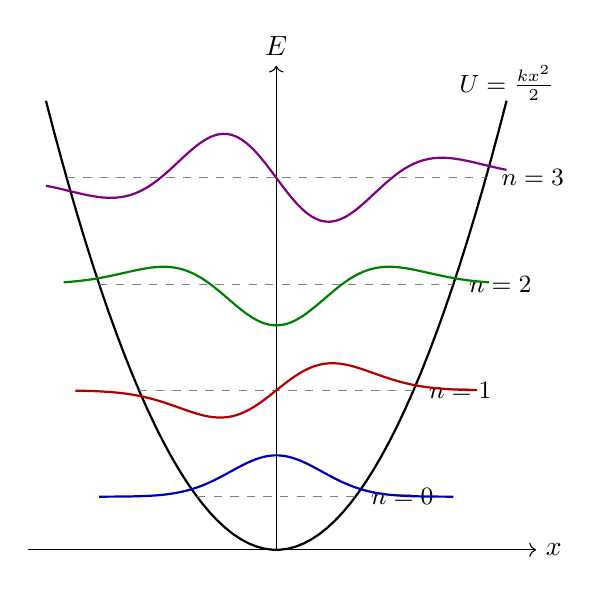
\begin{tikzpicture}[scale=0.75]
  \draw[->] (-4.2,0) -- (4.4,0) node[right]{$x$};
  \draw[->] (0,0) -- (0,8.2) node[above]{$E$};
  \draw[thick,domain=-3.9:3.9,samples=60] plot (\x,{0.5*\x*\x});
  \node[font=\small] at (3.9,7.9) {$U=\tfrac{kx^2}{2}$};
  \foreach \n/\c in {0/blue!70!black,1/red!70!black,2/green!50!black,3/violet}{
    \pgfmathsetmacro{\E}{1.8*\n+0.9}
    \pgfmathsetmacro{\xt}{sqrt(2*\E)}
    \draw[dashed,gray] (-\xt,\E) -- (\xt,\E);
    \node[right,font=\small] at (\xt+0.1,\E) {$n=\n$};
  }
  \draw[blue!70!black,thick,domain=-3:3,samples=80] plot (\x,{0.9+0.7*exp(-\x*\x/1.2)});
  \draw[red!70!black,thick,domain=-3.4:3.4,samples=80] plot (\x,{2.7+0.8*\x*exp(-\x*\x/1.8)});
  \draw[green!50!black,thick,domain=-3.6:3.6,samples=80] plot (\x,{4.5+0.35*(-2+1.6*\x*\x)*exp(-\x*\x/2.4)});
  \draw[violet,thick,domain=-3.9:3.9,samples=100] plot (\x,{6.3+0.18*(-12*\x/1.6+8*(\x/1.6)^3)*exp(-\x*\x/3.2)});
\end{tikzpicture}
\caption{Niveles igualmente espaciados del oscilador y las formas de $\varphi_n$ (esquemático).}
\end{figure}

\begin{obs}
Los $\Phi$ obtenidos son exactamente los polinomios de Hermite $H_n(\xi)$. Los niveles están igualmente espaciados
($\Delta E=\hbar\omega$) y la energía mínima no es cero («energía de punto cero»), coherente con el principio de
incertidumbre. Recuerda que $\xi=\sqrt\alpha\,x$, con $\sqrt\alpha=\sqrt{m\omega/\hbar}$.
\end{obs}

Al final de esta parte el cuaderno incluye dos esquemas: una función de onda que decae al entrar en una pared de
potencial y un pozo finito con un punto $x_1$ marcado (la penetración de $\varphi$ más allá del punto de retorno clásico).

% ============================================================
\section{Átomo de hidrógeno \pags{50--51}}
% ============================================================

\[
U=-\frac{e^2}{4\pi\varepsilon_0r}
\]
Por la forma del movimiento: coordenadas esféricas $(r,\theta,\phi)$.
\[
\nabla^2=\frac{1}{r^2}\frac{\partial}{\partial r}\left(r^2\frac{\partial}{\partial r}\right)
+\frac{1}{r^2\sen\theta}\frac{\partial}{\partial\theta}\left(\sen\theta\frac{\partial}{\partial\theta}\right)
+\frac{1}{r^2\sen^2\theta}\frac{\partial^2}{\partial\phi^2}
\]
\[
\hat H\varphi=E\varphi,\quad \varphi=\varphi(r,\theta,\phi):\qquad
\left(-\frac{\hbar^2}{2m}\nabla^2-\frac{e^2}{4\pi\varepsilon_0r}\right)\varphi=E\varphi
\]
\textbf{Separación de variables:} $\varphi(r,\theta,\phi)=R(r)\cdot\Theta(\theta)\cdot\Phi(\phi)$. Reemplazamos y dividimos entre $R\Theta\Phi$:
\[
\underbrace{\qquad\qquad}_{\substack{\text{de }r\\ -l(l+1)}}+\underbrace{\qquad\qquad}_{\substack{\text{de }\theta\text{ y }\phi\\ +l(l+1)}}=0
\quad\Longrightarrow\quad
\underbrace{\qquad\qquad}_{\substack{\text{de }\theta\\ m_l^2}}+\underbrace{\qquad\qquad}_{\substack{\text{de }\phi\\ -m_l^2}}=0
\]
Obtenemos:
\[
\frac1R\frac{d}{dr}\left(r^2\frac{dR}{dr}\right)+\frac{2mr^2}{\hbar^2}\left(E+\frac{e^2}{4\pi\varepsilon_0r}\right)=-l(l+1)\qquad(1)
\]
\[
\frac{\sen\theta}{\Theta}\frac{d}{d\theta}\left(\sen\theta\frac{d\Theta}{d\theta}\right)-l(l+1)\sen^2\theta=m_l^2\qquad(2)
\]
\[
\frac1\Phi\frac{d^2\Phi}{d\phi^2}=-m_l^2\qquad(3)
\]

\begin{obs}
El signo de la constante está invertido. Para llegar a los polinomios de Legendre y a $L^2=\hbar^2l(l+1)$, la parte radial
debe ser igual a $\boldsymbol{+l(l+1)}$ y la ecuación (2) queda con $\boldsymbol{+l(l+1)\sen^2\theta}=m_l^2$.
\end{obs}

\textbf{Solución de (3):} $\Phi=A\sen(m_l\phi)$. Si se da una vuelta ($\phi\to\phi+2\pi$), $\Phi(\phi+2\pi)=\Phi(\phi)$:
\[
A\sen[m_l(\phi+2\pi)]=A\sen(m_l\phi)\ \Rightarrow\ A\sen[m_l\phi+m_l2\pi]=A\sen(m_l\phi)
\]
$m_l\cdot2\pi$ debe ser múltiplo de $2\pi$ $\Rightarrow$ $m_l$ es entero: $m_l=0,\pm1,\pm2,\pm3,\ldots$

\begin{obs}
La solución general de (3) es $\Phi=A\,e^{im_l\phi}$ (o una combinación de seno y coseno). Se prefiere la exponencial porque
es función propia de $\hat L_z$; el seno solo no lo es. La conclusión ($m_l$ entero) es la misma.
\end{obs}

\textbf{Solución de (2):} en términos de los polinomios de Legendre asociados $P_{l\,m_l}(\cos\theta)$. De las propiedades
de estos polinomios: $l$ es entero y $l\ge|m_l|$.

\begin{center}
\begin{tabular}{cl}
\toprule
$l$ & $m_l$\\
\midrule
0 & 0\\
1 & $-1,\ 0,\ +1$\\
2 & $-2,\ -1,\ 0,\ +1,\ +2$\\
\bottomrule
\end{tabular}
\end{center}
Un estado dado por $l$ tiene un orden de degeneración de $(2l+1)$.

\textbf{Solución de (1):} en términos de los polinomios de Laguerre:
\[
R_{nl}=e^{-ar}\,r^l\,L_{nl}(r)
\]
De las propiedades de estos polinomios: $n$ es entero y $n\ge l+1$.

\begin{center}
\begin{tabular}{cl}
\toprule
$n$ & $l$\\
\midrule
1 & 0\\
2 & 0, 1\\
3 & 0, 1, 2\\
\bottomrule
\end{tabular}
\end{center}
\begin{itemize}
  \item $n$: número cuántico principal (total).
  \item $l$: número cuántico orbital.
  \item $m_l$: número cuántico magnético.
\end{itemize}

\subsection{Número cuántico principal}
\[
E=\frac{-me^4}{32\pi^2\varepsilon_0^2\hbar^2n^2}\qquad\text{(coincide con el resultado de Bohr).}
\]

\subsection{Número cuántico orbital}
$\hat L=\hat r\times\hat p$. Aplicamos $\hat L^2$ a $Y=\Theta\Phi$ y obtenemos:
\[
\hat L^2Y=\hbar^2\,l(l+1)\,Y\ \Rightarrow\ \boxed{L=\hbar\sqrt{l(l+1)}}
\]

\subsection{Número cuántico magnético}
Tomamos $\hat L_z=-i\hbar\,\partial/\partial\phi$ y aplicamos a $\varphi$: $\hat L_z\varphi=L_z\varphi$.
Solución: $\varphi=f(r,\theta)\cdot A\sen\!\left(\frac{L_z}{\hbar}\phi\right)$.

Luego de 1 vuelta ($\phi\to\phi+2\pi$):
\[
f(r,\theta)A\sen\!\left[\frac{L_z}{\hbar}(\phi+2\pi)\right]=f(r,\theta)A\sen\!\left(\frac{L_z}{\hbar}\phi\right)
\ \Rightarrow\
\sen\!\left[\frac{L_z}{\hbar}\phi+\frac{L_z}{\hbar}2\pi\right]=\sen\!\left(\frac{L_z}{\hbar}\phi\right)
\]
Múltiplo de $2\pi$: $L_z/\hbar=m_l$ $\rightarrow$ entero:
\[
\boxed{L_z=m_l\hbar}
\]

% ============================================================
\section{Momento magnético y efecto Zeeman \pags{51--52}}
% ============================================================

\subsection{Momento magnético del átomo de H (o momento dipolar magnético)}
Dipolo: espira de área $S$ con corriente $i$ $\rightarrow$ $\mu=iS$. El electrón ($-e$) en órbita genera una corriente $i=\nu e$:
\[
\mu=iS=\nu e\,\pi r^2
\]
Momento angular:
\[
L=rp=rm(\omega r)=rm(2\pi\nu r)=2mr^2\pi\nu
\ \Rightarrow\
\frac{\mu}{L}=\frac{e}{2m}\ \rightarrow\ \boxed{\vec\mu=-\frac{e}{2m}\vec L}
\]
($\vec\mu$ y $\vec L$ apuntan en sentidos opuestos porque la carga del electrón es negativa.)

\subsection{Efecto Zeeman}
Es la separación (desdoblamiento) de una línea espectral (de la emisión de los elementos: átomo aislado, estado gaseoso)
en varias, cuando el átomo está en un campo $\vec B$. Tomemos el átomo de H ($\vec B$ en la dirección $z$, $\vec L$ formando
un ángulo $\theta$ con $\vec B$).

Al colocar el átomo en un campo $\vec B$ $\Rightarrow$ interacción del átomo (dipolo) con $\vec B$:
\[
\vec\tau=\vec\mu\times\vec B,\qquad U=-\vec\mu\cdot\vec B
\]
\[
U=-|\vec\mu||\vec B|\cos(180^\circ-\theta)=-\frac{e}{2m}|\vec L||\vec B|(-\cos\theta)=\frac{e}{2m}|\vec B|\underbrace{|\vec L|\cos\theta}_{L_z=m_l\hbar}
\]
\[
\boxed{U=m_l\,\mu_B\,|\vec B|},\qquad \mu_B=\frac{e\hbar}{2m}\ \ (\text{magnetón de Bohr})
\]
\[
E=\frac{-me^4}{32\pi^2\varepsilon_0^2\hbar^2n^2}+m_l\mu_BB
\]

\textbf{Estados por nivel (diagrama del cuaderno):}
\begin{center}
\begin{tabular}{cll}
\toprule
$n$ & $l$ & $m_l$\\
\midrule
1 & 0 & 0\\
2 & 0, 1, 1, 1 & 0, $-1$, 0, 1\\
3 & 0, 1, 1, 1, 2, 2, 2, 2, 2 & 0, $-1$, 0, 1, $-2$, $-1$, 0, 1, 2\\
\bottomrule
\end{tabular}
\end{center}

\begin{figure}[H]
\centering
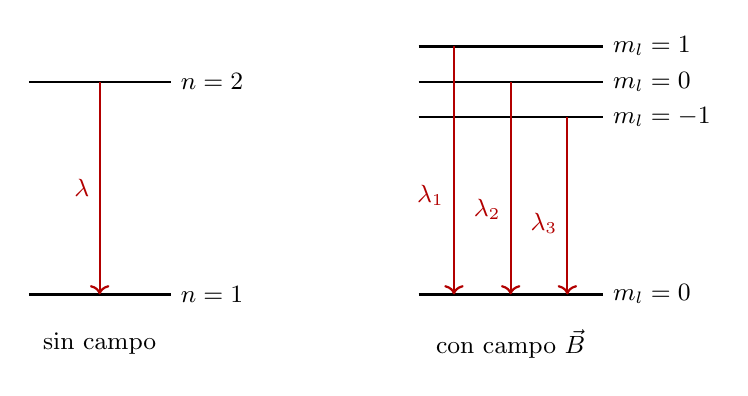
\begin{tikzpicture}[scale=0.9]
  % sin campo
  \draw[thick] (0,3) -- (2,3) node[right,font=\small]{$n=2$};
  \draw[thick] (0,0) -- (2,0) node[right,font=\small]{$n=1$};
  \draw[->,red!70!black,thick] (1,3) -- (1,0) node[midway,left,font=\small]{$\lambda$};
  \node[font=\small] at (1,-0.7) {sin campo};
  % con campo
  \begin{scope}[xshift=5.5cm]
  \draw[thick] (0,3.5) -- (2.6,3.5) node[right,font=\small]{$m_l=1$};
  \draw[thick] (0,3) -- (2.6,3) node[right,font=\small]{$m_l=0$};
  \draw[thick] (0,2.5) -- (2.6,2.5) node[right,font=\small]{$m_l=-1$};
  \draw[thick] (0,0) -- (2.6,0) node[right,font=\small]{$m_l=0$};
  \draw[->,red!70!black,thick] (0.5,3.5) -- (0.5,0) node[pos=0.6,left,font=\small]{$\lambda_1$};
  \draw[->,red!70!black,thick] (1.3,3) -- (1.3,0) node[pos=0.6,left,font=\small]{$\lambda_2$};
  \draw[->,red!70!black,thick] (2.1,2.5) -- (2.1,0) node[pos=0.6,left,font=\small]{$\lambda_3$};
  \node[font=\small] at (1.3,-0.7) {con campo $\vec B$};
  \end{scope}
\end{tikzpicture}
\caption{Efecto Zeeman: la transición $n=2\to n=1$ se separa en tres líneas.}
\end{figure}

\begin{obs}
Un valor útil: $\mu_B=9{,}27\times10^{-24}$ J/T $\approx5{,}79\times10^{-5}$ eV/T.
\end{obs}

% ============================================================
\section{Spin del electrón, principio de Pauli y reglas de selección \pags{52--53}}
% ============================================================

\textbf{Spin:} rotación alrededor de un eje propio.

La emisión más intensa del sodio es la transición $3p\to3s$. Pero, con un instrumento de mayor resolución, se detectaron
dos líneas cercanas ($\lambda_1$, $\lambda_2$).

Notación: $s\to l=0$, \ $p\to l=1$, \ $d\to l=2$, \ $f\to l=3$.

Tres situaciones:
\begin{itemize}
  \item Un átomo aislado con 1 solo e$^-$.
  \item Un átomo aislado con varios e$^-$.
  \item Varios átomos con varios e$^-$ (sólido).
\end{itemize}
En un átomo aislado con varios e$^-$, se quita cierta degeneración por la interacción de los e$^-$ entre sí: en el átomo H
los niveles $2s$ y $2p$ (o $3s$, $3p$, $3d$) coinciden; en el átomo con varios e$^-$ se separan.

Debe ser análogo al efecto Zeeman $\Rightarrow$ busquemos el dipolo y el campo.

\textbf{Dirac:} movimiento relativo del protón respecto al electrón (átomo H). Visto desde el e$^-$, el protón (e$^+$) gira a su
alrededor. En el centro de la circunferencia:
\[
B=\frac{\mu_0i}{2r}=\frac{\mu_0e\nu}{2r}
\]
Solo el e$^-$ puede ser el dipolo $\Rightarrow$ debe ser una esfera con spin (rotación), con momento angular $\vec L_s$ y momento
magnético $\vec\mu_s$ opuestos:
\[
\frac{\mu_s}{L_s}=\frac{\gamma e}{2m},\qquad \vec\mu_s=-\frac{e\gamma}{2m}\vec L_s
\]
$\gamma$: razón giratoria magnética ($\gamma=2{,}004$).

\begin{obs}
El valor medido del factor $g$ del electrón es $2{,}0023$ (la teoría de Dirac predice exactamente 2). Históricamente, el spin
lo propusieron Uhlenbeck y Goudsmit (1925); Dirac lo dedujo de su ecuación relativista (1928).
\end{obs}

Dirac desarrolló una teoría y obtuvo:
\[
L_s=\hbar\sqrt{s(s+1)},\qquad L_{sz}=m_s\hbar,\qquad s=\tfrac12,\quad m_s=-\tfrac12,\ \tfrac12
\]
$m_s$: número cuántico magnético de spin.
\[
U=-\vec\mu_s\cdot\vec B=-\left(-\frac{e\gamma}{2m}\vec L_s\right)\cdot\vec B=\frac{e\gamma}{2m}L_sB\cos\theta=\frac{e\gamma}{2m}BL_{sz}=\frac{e\gamma}{2m}Bm_s\hbar
\]
\[
\boxed{U=m_s\,\mu_B\,B\,\gamma}
\]

\begin{figure}[H]
\centering
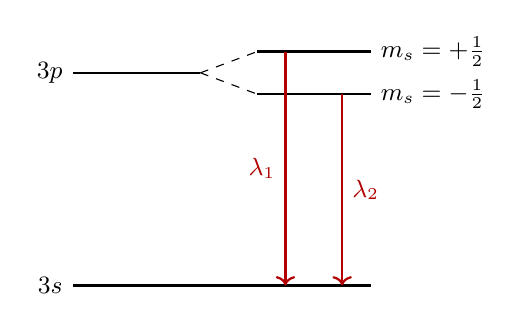
\begin{tikzpicture}[scale=0.9]
  \draw[thick] (0,3) -- (1.8,3) node[pos=0,left,font=\small]{$3p$};
  \draw[thick] (2.6,3.3) -- (4.2,3.3) node[right,font=\small]{$m_s=+\tfrac12$};
  \draw[thick] (2.6,2.7) -- (4.2,2.7) node[right,font=\small]{$m_s=-\tfrac12$};
  \draw[dashed] (1.8,3) -- (2.6,3.3); \draw[dashed] (1.8,3) -- (2.6,2.7);
  \draw[thick] (0,0) -- (4.2,0) node[pos=0,left,font=\small]{$3s$};
  \draw[->,red!70!black,thick] (3.0,3.3) -- (3.0,0) node[pos=0.5,left,font=\small]{$\lambda_1$};
  \draw[->,red!70!black,thick] (3.8,2.7) -- (3.8,0) node[pos=0.5,right,font=\small]{$\lambda_2$};
\end{tikzpicture}
\caption{El nivel $3p$ del sodio se desdobla en $m_s=\pm\tfrac12$: la transición a $3s$ da dos líneas (doblete).}
\end{figure}

\textbf{Un estado está determinado por 4 números cuánticos: $n$, $l$, $m_l$, $m_s$.}

\subsection{Principio de exclusión de Pauli}
En cada estado descrito por los 4 números cuánticos no puede haber más de un electrón.

Ejemplo del cuaderno: $n=1$ ($l=0$, $m_l=0$) admite $\uparrow\downarrow$; en $n=2$, el $2s$ admite $\uparrow\downarrow$ y el
$2p$ tiene tres orbitales ($m_l=-1,0,1$), cada uno con hasta $\uparrow\downarrow$.

\subsection{Reglas de selección}
Se evalúa la probabilidad de cada posible transición. Algunas son muy pequeñas (equivale a una transición prohibida).
Ha derivado en las siguientes reglas de selección. Transiciones permitidas si:
\[
\boxed{\Delta l=\pm1,\qquad \Delta m_l=-1,\ 0,\ 1}
\]
Ejemplo: de $n=3$ ($l=2$, $m_l=-2$) a $n=2$ ($l=1$, $m_l=-1$): $\Delta l=1-2=-1$ \checkmark, \
$\Delta m_l=-1-(-2)=1$ \checkmark\ $\rightarrow$ permitida.

\subsection{Niveles de energía según el sistema}
\begin{figure}[H]
\centering
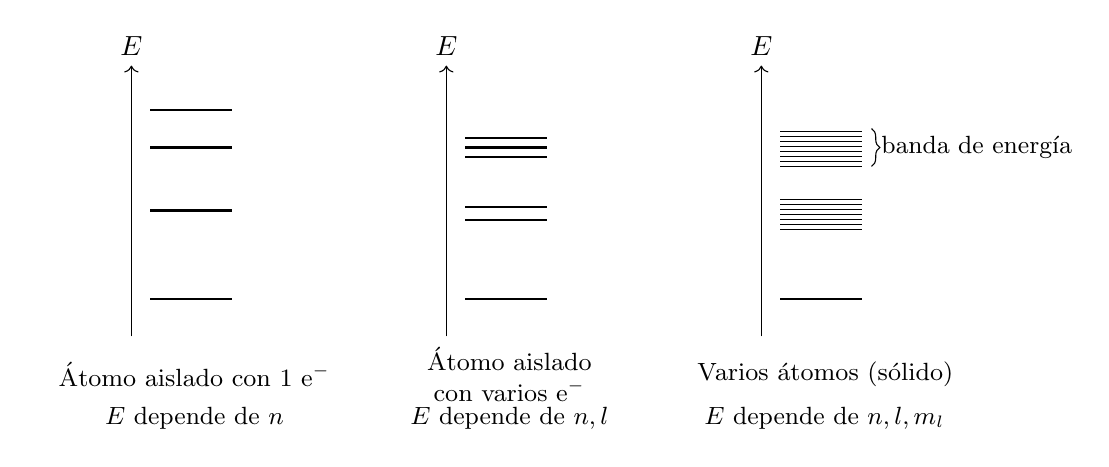
\begin{tikzpicture}[scale=0.8]
  \foreach \i/\t/\d in {0/{Átomo aislado con 1 e$^-$}/{$n$},1/{Átomo aislado con varios e$^-$}/{$n,l$},2/{Varios átomos (sólido)}/{$n,l,m_l$}}{
    \begin{scope}[xshift=\i*5cm]
      \draw[->] (0,0) -- (0,4.3) node[above]{$E$};
      \node[font=\small,align=center,text width=4cm] at (1,-0.6) {\t};
      \node[font=\small] at (1,-1.3) {$E$ depende de \d};
    \end{scope}}
  \foreach \y in {0.6,2.0,3.0,3.6} \draw[thick] (0.3,\y) -- (1.6,\y);
  \begin{scope}[xshift=5cm]
    \draw[thick] (0.3,0.6) -- (1.6,0.6);
    \foreach \y in {1.85,2.05} \draw[thick] (0.3,\y) -- (1.6,\y);
    \foreach \y in {2.85,3.0,3.15} \draw[thick] (0.3,\y) -- (1.6,\y);
  \end{scope}
  \begin{scope}[xshift=10cm]
    \draw[thick] (0.3,0.6) -- (1.6,0.6);
    \foreach \y in {1.7,1.78,...,2.2} \draw[line width=0.25pt] (0.3,\y) -- (1.6,\y);
    \foreach \y in {2.7,2.78,...,3.3} \draw[line width=0.25pt] (0.3,\y) -- (1.6,\y);
    \draw[decorate,decoration={brace,amplitude=3pt}] (1.75,3.3) -- (1.75,2.7) node[midway,right,font=\small]{banda de energía};
  \end{scope}
\end{tikzpicture}
\caption{Del átomo aislado al sólido: los niveles se abren en subniveles y luego en bandas.}
\end{figure}
% ============================================================
\section{Cristalografía \pags{53--57}}
% ============================================================

% Cubo en proyección oblicua: \cubo{escala}
\tikzset{
  cubo/.pic={
    \coordinate (A) at (0,0); \coordinate (B) at (1,0); \coordinate (C) at (1,1); \coordinate (D) at (0,1);
    \coordinate (E) at (0.4,0.3); \coordinate (F) at (1.4,0.3); \coordinate (G) at (1.4,1.3); \coordinate (H) at (0.4,1.3);
    \draw (A)--(B)--(C)--(D)--cycle; \draw (B)--(F)--(G)--(C); \draw (D)--(H)--(G);
    \draw[dashed] (A)--(E)--(F); \draw[dashed] (E)--(H);
  }
}

Los sólidos pueden ser \textbf{cristalinos} o \textbf{amorfos}.

\textbf{Cristal:} sólido anisótropo cuyas moléculas, átomos o iones están dispuestos en forma ordenada formando figuras
geométricas definidas.

\textbf{Red cristalina:} arreglo de puntos que resulta al reemplazar cada átomo (molécula o ion) por un punto.

\textbf{Base (de la sustancia):} aquello a lo que representa cada punto de la red.

\begin{center}
\textbf{RED + BASE = CRISTAL}
\end{center}

\subsection{Algunas definiciones}
\begin{itemize}
  \item \textbf{Celda unitaria:} porción más pequeña con cuya repetición se forma el cristal.
  \item \textbf{Estructura simple:} hay puntos solo en los vértices del paralelogramo que es la celda.
  \item \textbf{Estructura no simple:} hay puntos también dentro de la celda. Se distingue la \emph{celda convencional} de la
        \emph{celda primitiva}.
  \item \textbf{Vectores base convencionales:} los que determinan la celda convencional $(\vec a,\vec b,\vec c)$.
  \item \textbf{Vectores base primitivos:} los que determinan la celda primitiva $(\vec a\,',\vec b\,',\vec c\,')$.
\end{itemize}

\begin{figure}[H]
\centering
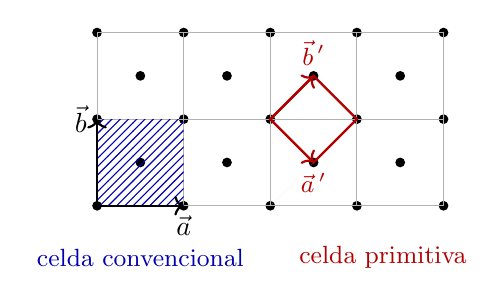
\begin{tikzpicture}[scale=1.1]
  \foreach \x in {0,...,4} \foreach \y in {0,...,2} \fill (\x,\y) circle (1.6pt);
  \foreach \x in {0,...,3} \foreach \y in {0,1} \fill (\x+0.5,\y+0.5) circle (1.6pt);
  \foreach \y in {0,...,2} \draw[gray!60] (0,\y) -- (4,\y);
  \foreach \x in {0,...,4} \draw[gray!60] (\x,0) -- (\x,2);
  \fill[pattern=north east lines,pattern color=blue!70!black] (0,0) rectangle (1,1);
  \draw[->,thick] (0,0) -- (1,0) node[below]{$\vec a$};
  \draw[->,thick] (0,0) -- (0,1) node[left]{$\vec b$};
  \fill[red!20,opacity=0.7] (2,0) -- (2.5,0.5) -- (3,1) -- (2.5,0.5) -- cycle;
  \draw[red!70!black,thick] (2,1) -- (2.5,0.5) -- (3,1) -- (2.5,1.5) -- cycle;
  \draw[->,red!70!black,thick] (2,1) -- (2.5,0.5) node[below,font=\small]{$\vec a\,'$};
  \draw[->,red!70!black,thick] (2,1) -- (2.5,1.5) node[above,font=\small]{$\vec b\,'$};
  \node[font=\small,blue!70!black] at (0.5,-0.6) {celda convencional};
  \node[font=\small,red!70!black] at (3.3,-0.6) {celda primitiva};
\end{tikzpicture}
\caption{Estructura no simple (2D): la celda convencional tiene 2 puntos; la primitiva, 1.}
\end{figure}

\subsection{Simetría cristalina}
Transformaciones de simetría: desplazamientos que vuelven a reproducir el cristal. Tenemos:
\begin{itemize}
  \item Simetría de traslación.
  \item Simetría de rotación alrededor de un eje.
  \item Simetría de reflexión en un plano.
  \item Simetría de inversión respecto a un punto.
\end{itemize}

\subsection{Redes de Bravais}
Las agruparemos en 7 sistemas, según las longitudes $a$, $b$, $c$ y los ángulos $\alpha$, $\beta$, $\gamma$ entre los vectores base.

\begin{center}
\begin{tabular}{llll}
\toprule
Sistema & Longitudes & Ángulos & Redes\\
\midrule
1. Cúbico & $a=b=c$ & $\alpha=\beta=\gamma=90^\circ$ & sc, bcc, fcc\\
2. Hexagonal & $a=b\neq c$ & $\alpha=\beta=90^\circ$, $\gamma=120^\circ$ & ---\\
\bottomrule
\end{tabular}
\end{center}

\begin{figure}[H]
\centering
\begin{tikzpicture}[scale=1.6]
  \pic at (0,0) {cubo};
  \foreach \p in {(0,0),(1,0),(1,1),(0,1),(0.4,0.3),(1.4,0.3),(1.4,1.3),(0.4,1.3)} \fill \p circle (1.2pt);
  \node at (0.7,-0.3) {sc};
  \begin{scope}[xshift=2.4cm]
  \pic at (0,0) {cubo};
  \foreach \p in {(0,0),(1,0),(1,1),(0,1),(0.4,0.3),(1.4,0.3),(1.4,1.3),(0.4,1.3)} \fill \p circle (1.2pt);
  \fill[red!70!black] (0.7,0.65) circle (1.5pt);
  \node at (0.7,-0.3) {bcc};
  \end{scope}
  \begin{scope}[xshift=4.8cm]
  \pic at (0,0) {cubo};
  \foreach \p in {(0,0),(1,0),(1,1),(0,1),(0.4,0.3),(1.4,0.3),(1.4,1.3),(0.4,1.3)} \fill \p circle (1.2pt);
  \foreach \p in {(0.5,0.5),(0.9,0.8),(0.2,0.65),(1.2,0.65),(0.7,0.15),(0.7,1.15)} \fill[red!70!black] \p circle (1.5pt);
  \node at (0.7,-0.3) {fcc};
  \end{scope}
\end{tikzpicture}
\caption{Sistema cúbico: sc (\emph{simple cube}), bcc (\emph{body centered cube}, cubo centrado en el cuerpo, CCC) y fcc (\emph{face centered cube}).}
\end{figure}

\begin{obs}
El cuaderno solo anota 2 de los 7 sistemas. Los otros cinco son tetragonal, ortorrómbico, romboedral (trigonal),
monoclínico y triclínico; en total hay 14 redes de Bravais.
\end{obs}

\subsection{Celda primitiva en las redes cúbicas}
\textbf{fcc}
\begin{center}
\renewcommand{\arraystretch}{1.3}
\begin{tabular}{ll}
\toprule
Vectores base & Vectores primitivos\\
\midrule
$\vec a=a\,\ii$ & $\vec a\,'=\frac12(\vec a+\vec b)=\frac a2(\ii+\jj)$\\
$\vec b=a\,\jj$ & $\vec b\,'=\frac12(\vec b+\vec c)=\frac a2(\jj+\kk)$\\
$\vec c=a\,\kk$ & $\vec c\,'=\frac12(\vec a+\vec c)=\frac a2(\ii+\kk)$\\
Volumen: $v=\vec a\cdot(\vec b\times\vec c)=a^3$ & Volumen: $v=\vec a\,'\cdot(\vec b\,'\times\vec c\,')=a^3/4$\\
\bottomrule
\end{tabular}
\end{center}
A una celda convencional le corresponden 4 puntos de la red: $(0,0,0)$, $(\tfrac a2,\tfrac a2,0)$, $(0,\tfrac a2,\tfrac a2)$, $(\tfrac a2,0,\tfrac a2)$.

\emph{Tomemos una estructura en 2 dimensiones:} correspondencia entre puntos y celdas $\rightarrow$ 1 punto a 1 celda (primitiva);
2 puntos $\rightarrow$ a una celda convencional.

\textbf{bcc}

Vectores base: los mismos. Vectores primitivos:
\[
\vec a\,'=\frac a2(-\ii+\jj+\kk),\qquad \vec b\,'=\frac a2(\ii-\jj+\kk),\qquad \vec c\,'=\frac a2(\ii+\jj-\kk),\qquad
v=\vec a\,'\cdot(\vec b\,'\times\vec c\,')=\frac{a^3}{2}
\]
2 puntos de la red $\rightarrow$ a 1 celda convencional: $(0,0,0)$, $(\tfrac a2,\tfrac a2,\tfrac a2)$.

\subsection{Fracción de empaquetamiento ($f$)}
\[
f=\frac{\parbox{9cm}{\centering volumen de los puntos correspondientes a la celda convencional,\\ tomados como esferas del mayor tamaño}}{\text{volumen de la celda}}
\]
\[
f_{sc}=\frac{1\left[\frac43\pi\left(\frac a2\right)^3\right]}{a^3},\qquad
f_{bcc}=\frac{2\left[\frac43\pi\left(\frac{a\sqrt3}{4}\right)^3\right]}{a^3},\qquad
f_{fcc}=\frac{4\left[\frac43\pi\left(\frac{a\sqrt2}{4}\right)^3\right]}{a^3}
\]
\begin{center}
\begin{tabular}{ccccc}
\toprule
Red & Puntos por celda & Radio máximo & $f$ (cuaderno) & $f$ (valor exacto)\\
\midrule
sc & 1 & $r=a/2$ & 0,56 & $\pi/6\approx0{,}52$\\
bcc & 2 & $r=a\sqrt3/4$ & 0,6 & $\pi\sqrt3/8\approx0{,}68$\\
fcc & 4 & $r=a\sqrt2/4$ & 0,7 & $\pi\sqrt2/6\approx0{,}74$\\
\bottomrule
\end{tabular}
\end{center}

\begin{obs}
Revisa los valores numéricos: los correctos son 0,52; 0,68 y 0,74 (columna de la derecha). Además, en la fórmula de fcc el
cuaderno escribe $(a\sqrt2/3)^3$; debe ser $(a\sqrt2/4)^3$, como el propio radio anotado al lado.
\end{obs}

\subsection{Algunas estructuras cristalinas}
\begin{center}
\footnotesize
\renewcommand{\arraystretch}{1.35}
\begin{tabularx}{\textwidth}{@{}l l >{\raggedright\arraybackslash}X l l >{\raggedright\arraybackslash}X@{}}
\toprule
Estructura & Red & Descripción & Puntos por celda conv. & $a$ & Otras sustancias\\
\midrule
NaCl & fcc & 2 fcc (Cl y Na) desplazadas en $\tfrac12a$. Base: Cl$(0,0,0)$, Na$(\tfrac a2,\tfrac a2,\tfrac a2)$ & 4 (4 moléculas) & 5,63 Å & LiH, KCl, AgBr, MgO, KBr\\
CsCl & sc & 2 sc (Cl y Cs) desplazadas en $\tfrac12$ diagonal. Base: Cl$(0,0,0)$, Cs$(\tfrac a2,\tfrac a2,\tfrac a2)$ & 1 (1 molécula) & 4,11 Å & AlNi, LiHg, AgMg, CuPd\\
Diamante & fcc & 2 fcc de átomos de C desplazadas en $\tfrac14$ diagonal. Base: C$(0,0,0)$, C$(\tfrac a4,\tfrac a4,\tfrac a4)$ & 4 (8 átomos) & 3,56 Å & Si, Ge\\
ZnS & fcc & Similar al diamante: 2 fcc (S y Zn) desplazadas en $\tfrac14$ diagonal. Base: S$(0,0,0)$, Zn$(\tfrac a4,\tfrac a4,\tfrac a4)$ & 4 (4 moléculas) & --- & CuF, CuCl, GaP, GaAs, CdS\\
\bottomrule
\end{tabularx}
\end{center}
($a,b,c$ $\rightarrow$ parámetros de la red.)

\subsection{Planos cristalinos o reticulares}
Se forman con los puntos de la red (los planos pasan por puntos de la red). ¿Cómo designaremos a un plano para
diferenciarlo de otro? Mediante los índices de Miller.

\textbf{Índices de Miller $(h,k,l)$:} $h$, $k$ y $l$ son enteros, tales que sus inversas $\left(\frac1h,\frac1k,\frac1l\right)$ son los
puntos en que el plano corta a los ejes cristalográficos.

\textbf{Ejes cristalográficos:} dirigidos a lo largo de los vectores base $\vec a,\vec b,\vec c$ $(x_0,y_0,z_0)$.

\begin{figure}[H]
\centering
\begin{tikzpicture}[scale=1.1]
  \draw[->] (0,0) -- (3,0) node[right]{$y_0$};
  \draw[->] (0,0) -- (0,2.8) node[above]{$z_0$};
  \draw[->] (0,0) -- (-1.5,-1.2) node[below left]{$x_0$};
  \coordinate (X) at (-1,-0.8); \coordinate (Y) at (2.2,0); \coordinate (Z) at (0,2.1);
  \fill[blue!15] (X) -- (Y) -- (Z) -- cycle; \draw[thick,blue!70!black] (X) -- (Y) -- (Z) -- cycle;
  \node[below,font=\small] at (X) {$\tfrac1h a$}; \node[below,font=\small] at (Y) {$\tfrac1k b$}; \node[left,font=\small] at (Z) {$\tfrac1l c$};
  \node[font=\small] at (0,-0.25) {O};
  \node[font=\small,blue!70!black] at (2.3,1.6) {«El plano» $(hkl)$};
\end{tikzpicture}
\caption{El plano $(hkl)$ corta los ejes en $a/h$, $b/k$ y $c/l$.}
\end{figure}

\begin{itemize}
  \item Otro plano (de la misma familia) pasa por el origen.
  \item «El plano» $\rightarrow$ plano más cercano al origen.
\end{itemize}

\textbf{Ejemplo:} dibuje los planos $(100)$, $(1\bar10)$, $(210)$, $(010)$ de una red cúbica.

\begin{center}
\begin{tabular}{ccc}
\toprule
Plano & Índices de Miller & Inversas (cortes con $x$, $y$, $z$)\\
\midrule
$(100)$ & $1,\ 0,\ 0$ & $1,\ \infty,\ \infty$\\
$(1\bar10)$ & $1,\ -1,\ 0$ & $1,\ -1,\ \infty$\\
$(210)$ & $2,\ 1,\ 0$ & $\tfrac12,\ 1,\ \infty$\\
$(010)$ & $0,\ 1,\ 0$ & $\infty,\ 1,\ \infty$\\
\bottomrule
\end{tabular}
\end{center}

\begin{figure}[H]
\centering
\begin{tikzpicture}[scale=1.5]
  % (100)
  \pic at (0,0) {cubo};
  \fill[blue!25,opacity=0.8] (0,0) -- (1,0) -- (1,1) -- (0,1) -- cycle;
  \node at (0.7,-0.3) {$(100)$};
  % (1-10)
  \begin{scope}[xshift=2.4cm]
  \pic at (0,0) {cubo};
  \fill[blue!25,opacity=0.8] (0,0) -- (1.4,0.3) -- (1.4,1.3) -- (0,1) -- cycle;
  \node at (0.7,-0.3) {$(1\bar10)$};
  \end{scope}
  % (210)
  \begin{scope}[xshift=4.8cm]
  \pic at (0,0) {cubo};
  \fill[blue!25,opacity=0.8] (0.2,0.15) -- (1,0) -- (1,1) -- (0.2,1.15) -- cycle;
  \node at (0.7,-0.3) {$(210)$};
  \end{scope}
  % (010)
  \begin{scope}[xshift=7.2cm]
  \pic at (0,0) {cubo};
  \fill[blue!25,opacity=0.8] (1,0) -- (1.4,0.3) -- (1.4,1.3) -- (1,1) -- cycle;
  \node at (0.7,-0.3) {$(010)$};
  \end{scope}
\end{tikzpicture}
\caption{Planos del ejemplo en una celda cúbica (esquemático; $x$ hacia el frente, $y$ a la derecha, $z$ hacia arriba).}
\end{figure}

\textbf{Familia de planos $\{h\,k\,l\}$.} Ej.: los planos $(100)$, $(010)$, $(001)$ forman la familia $\{100\}$.

\textbf{Direcciones $[h\,k\,l]$:} una dirección $[hkl]$ es una recta a lo largo del vector $\vec r=h\vec a+k\vec b+l\vec c$.
Familia de direcciones: $\langle h\,k\,l\rangle$.

\subsection{Distancia interplanar (red con $\alpha=\beta=\gamma=90^\circ$)}
\begin{minipage}{0.4\textwidth}
\centering
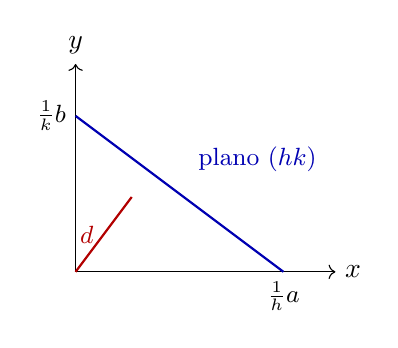
\begin{tikzpicture}[scale=1.1]
  \draw[->] (0,0) -- (3,0) node[right]{$x$};
  \draw[->] (0,0) -- (0,2.4) node[above]{$y$};
  \draw[thick,blue!70!black] (2.4,0) -- (0,1.8);
  \node[below,font=\small] at (2.4,0) {$\tfrac1h a$};
  \node[left,font=\small] at (0,1.8) {$\tfrac1k b$};
  \draw[red!70!black,thick] (0,0) -- (0.648,0.864) node[midway,left,font=\small]{$d$};
  \node[font=\small,blue!70!black] at (2.1,1.3) {plano $(hk)$};
\end{tikzpicture}
\end{minipage}\hfill
\begin{minipage}{0.55\textwidth}
En 2D, por semejanza de triángulos:
\[
\frac{d}{a/h}=\frac{b/k}{\sqrt{(a/h)^2+(b/k)^2}}
\ \Rightarrow\
d=\frac{1}{\sqrt{(h/a)^2+(k/b)^2}}
\]
\end{minipage}

En 3 dimensiones:
\[
\boxed{d=\frac{1}{\sqrt{\left(\frac ha\right)^2+\left(\frac kb\right)^2+\left(\frac lc\right)^2}}}
\]

% ============================================================
\section{Difracción de rayos X y red recíproca \pags{57--59}}
% ============================================================

\subsection{Ley de Bragg}
Bragg: difracción por reflexión en los planos cristalinos.

\begin{figure}[H]
\centering
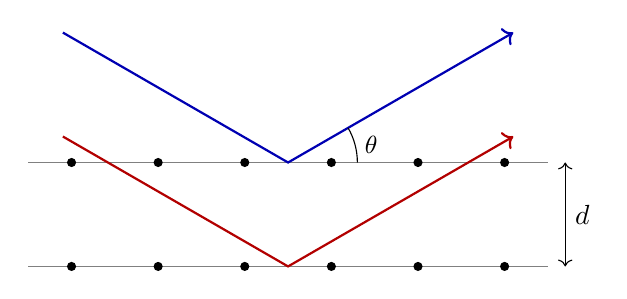
\begin{tikzpicture}[scale=1.1]
  \foreach \y in {0,-1.2} {\draw[gray] (-3,\y) -- (3,\y); \foreach \x in {-2.5,-1.5,...,2.5} \fill (\x,\y) circle (1.5pt);}
  \draw[->,thick,blue!70!black] (-2.6,1.5) -- (0,0) -- (2.6,1.5);
  \draw[->,thick,red!70!black] (-2.6,0.3) -- (0,-1.2) -- (2.6,0.3);
  \draw (0.8,0) arc (0:30:0.8) node[midway,right,font=\small]{$\theta$};
  \draw[<->] (3.2,0) -- (3.2,-1.2) node[midway,right]{$d$};
\end{tikzpicture}
\caption{Reflexión de rayos X en dos planos vecinos separados una distancia $d$.}
\end{figure}

Diferencia de camino:
\[
\Delta=\frac{d}{\sen\theta}+\frac{d}{\sen\theta}-2d\cot\theta\,\cos\theta=\frac{2d}{\sen\theta}(1-\cos^2\theta)=2d\sen\theta
\]

\begin{obs}
En el cuaderno el tercer término aparece como $\dfrac{2d}{\cot\theta}\cos\theta$; debe ser $2d\cot\theta\cos\theta$ (o
$\dfrac{2d}{\tan\theta}\cos\theta$) para que salga la línea siguiente, que sí está bien.
\end{obs}

Para un máximo de difracción: $\Delta=n\lambda$, $n=1,2,3,\ldots$
\[
\boxed{n\lambda=2d\sen\theta}\qquad(\text{ley de Bragg}),\qquad n\rightarrow\text{orden de difracción.}
\]

\subsection{Determinación de la estructura cristalina}
Se hace por métodos de difracción de rayos X.
\begin{itemize}
  \item \textbf{Método de Debye--Scherrer.} Muestra: polvo de cristales. Los rayos difractados forman conos de semiángulo
        $2\theta$, que en la pantalla (o en una película enrollada alrededor de la muestra) se ven como anillos, uno por cada
        orden ($n=1$, $n=2$, \ldots).
  \item \textbf{Método de Laue.} Muestra: monocristal. En la pantalla aparece un patrón de puntos, que representa la
        red recíproca.
\end{itemize}

\subsection{Método de Laue para la amplitud de la onda dispersada}
Toma a cada punto de la red como un centro dispersor (como fuente puntual).
\[
\vec\rho_{mnp}=m\vec a+n\vec b+p\vec c\qquad(m,n,p:\ \text{enteros};\ \vec a,\vec b,\vec c:\ \text{vectores base})
\]
Campo eléctrico de la onda incidente:
\[
E_i=E_0\,e^{i(\vec k\cdot\vec\rho_{mnp}-\omega t)}
\]
Onda dispersada en el punto de la pantalla:
\[
E_d=C\,\frac{E_i}{r}\,e^{i\vec k\,'\cdot\vec r}
\]
Consideramos $|\vec k\,'|=|\vec k|=k$.

\textbf{Aproximaciones:}
\begin{itemize}
  \item En el denominador: $r\approx R$.
  \item En $e^{i\vec k\,'\cdot\vec r}$ no podemos hacer $\vec r\approx\vec R$: $\frac{1}{1\,\text{Å}}(1\ \text{m})$ y
        $\frac{1}{1\,\text{Å}}(1\ \text{m}+1\ \text{Å})$ difieren en un desfase de 1 rad.
\end{itemize}
\[
R\approx r+\rho_{mnp}\cos\theta\ \Rightarrow\ r=R-\rho_{mnp}\cos\theta,\qquad
\vec k\,'\cdot\vec r=|\vec k\,'||\vec r|\cos0^\circ=kr=k(R-\rho_{mnp}\cos\theta)
\]
\[
E_d=\frac CR\,e^{i(\vec k\cdot\vec\rho_{mnp}-\omega t)}\cdot e^{ikR-\overbrace{ik\rho_{mnp}\cos\theta}^{i\vec k\,'\cdot\vec\rho_{mnp}}},
\qquad \Delta\vec k=\vec k\,'-\vec k
\]
\[
E_d=\underbrace{\frac CR\,e^{ikR}e^{-i\omega t}}_{\text{no cambia}}\cdot\underbrace{e^{-i\Delta\vec k\cdot\vec\rho_{mnp}}}_{\text{«amplitud»}}
\]
Amplitud del campo eléctrico de la onda dispersada (difundida) por el punto de la red en $\vec\rho_{mnp}$:
$e^{-i\Delta\vec k\cdot\vec\rho_{mnp}}$. Por todos los puntos de la red:
\[
A=\sum_{mnp}e^{-i\Delta\vec k\cdot\vec\rho_{mnp}}
\]
\textbf{Condición de difracción:} que $A$ sea máxima. En particular, cuando cada término de la sumatoria toma su valor máximo:
\[
e^{-i\Delta\vec k\cdot\vec\rho_{mnp}}\rightarrow\text{máx}\ \Rightarrow\
\boxed{\Delta\vec k\cdot\vec\rho_{mnp}=\text{entero}\times(2\pi)}\quad(\text{nueva forma de la ley de Bragg})
\]
Es equivalente a las \textbf{ecuaciones de Laue}:
\[
\Delta\vec k\cdot\vec a=2\pi h,\qquad \Delta\vec k\cdot\vec b=2\pi k,\qquad \Delta\vec k\cdot\vec c=2\pi l
\]
\[
\Delta\vec k\cdot(m\vec a+n\vec b+p\vec c)=m\,\Delta\vec k\cdot\vec a+n\,\Delta\vec k\cdot\vec b+p\,\Delta\vec k\cdot\vec c=2\pi(\text{entero})
\]
Debemos resolver las ecuaciones para hallar $\Delta\vec k$. Solución trivial, cuando $\vec a$, $\vec b$ y $\vec c$ son perpendiculares:
\[
\Delta\vec k=2\pi\left(\frac ha\hat u_a+\frac kb\hat u_b+\frac lc\hat u_c\right)
\]
Para otros casos necesitamos la red recíproca.

\subsection{Red recíproca}
A la que hemos visto antes la llamamos \textbf{red directa} (vectores $\vec a,\vec b,\vec c$); la recíproca tiene vectores $\vec A,\vec B,\vec C$.

Relación entre una red (directa) y su recíproca ($\vec a,\vec b,\vec c$ y $\vec A,\vec B,\vec C$: vectores primitivos):
\[
\begin{array}{lll}
\vec A\cdot\vec a=2\pi & \vec B\cdot\vec a=0 & \vec C\cdot\vec a=0\\
\vec A\cdot\vec b=0 & \vec B\cdot\vec b=2\pi & \vec C\cdot\vec b=0\\
\vec A\cdot\vec c=0 & \vec B\cdot\vec c=0 & \vec C\cdot\vec c=2\pi
\end{array}
\]
Para 3 dimensiones se ha obtenido:
\[
\vec A=\frac{2\pi}{v}(\vec b\times\vec c),\qquad \vec B=\frac{2\pi}{v}(\vec c\times\vec a),\qquad \vec C=\frac{2\pi}{v}(\vec a\times\vec b),\qquad
v=\vec a\cdot(\vec b\times\vec c)
\]

\textbf{Ejemplo: halle la red recíproca de una sc.} \ $\vec a=a\ii$, $\vec b=b\jj$, $\vec c=c\kk$, \ $v=a^3$:
\[
\vec A=\frac{2\pi}{v}(\vec b\times\vec c)=\frac{2\pi}{a^3}a^2\ii=\frac{2\pi}{a}\ii,\qquad
\vec B=\frac{2\pi}{a}\jj,\qquad \vec C=\frac{2\pi}{a}\kk
\]
$\rightarrow$ La red recíproca es una sc de parámetro $2\pi/a$.

\begin{obs}
En el cuaderno se escribe $\vec b=b\jj$ y $\vec c=c\kk$ pero se calcula con $v=a^3$, es decir, tomando $a=b=c$ (que es lo
que corresponde a una sc).
\end{obs}

\textbf{Ejemplo: halle la red recíproca de una fcc.}\
$\vec a\,'=\frac a2(\ii+\jj)$, $\vec b\,'=\frac a2(\jj+\kk)$, $\vec c\,'=\frac a2(\ii+\kk)$, \ $v=\vec a\,'\cdot(\vec b\,'\times\vec c\,')=\frac{a^3}{4}$:
\[
\vec A\,'=\frac{2\pi}{v}(\vec b\,'\times\vec c\,')=\frac{2\pi}{a^3/4}\cdot\frac{a^2}{4}(-\kk+\ii+\jj)=\frac{2\pi}{a}(\ii+\jj-\kk)
\]
\[
\vec B\,'=\frac{2\pi}{v}(\vec c\,'\times\vec a\,')=\frac{2\pi}{a}(-\ii+\jj+\kk),\qquad
\vec C\,'=\frac{2\pi}{v}(\vec a\,'\times\vec b\,')=\frac{2\pi}{a}(\ii-\jj+\kk)
\]
$\rightarrow$ La recíproca de una fcc es una bcc.

\subsection{Propiedades de la red recíproca}
\begin{enumerate}
  \item Todo vector $\vec G_{hkl}$ de la red recíproca es $\perp$ a los planos $(hkl)$ de la red directa, donde
        $\vec G_{hkl}=h\vec A+k\vec B+l\vec C$.
  \item $|\vec G_{hkl}|=\dfrac{2\pi}{d_{hkl}}$ \quad ($d_{hkl}$: distancia entre los planos $(hkl)$ de la red directa).
  \item $V=\dfrac{(2\pi)^3}{v}$ \quad ($v$: volumen de la celda primitiva en la red directa; $V$: en la red recíproca).
\end{enumerate}

\subsection{Volvamos a la condición de difracción}
$\Delta\vec k\cdot\vec\rho_{mnp}=\text{entero}\times2\pi$, o ecuaciones de Laue. La solución trivial era un caso particular.
En general, $\Delta\vec k$ debe ser un vector cualquiera de la red recíproca:
\[
\boxed{\Delta\vec k=\vec G}\ \ (\text{o }\vec G_{hkl})\qquad(\text{otra forma de la ley de Bragg})
\]
Veamos la relación con $n\lambda=2d\sen\theta$ ($\vec k\,'$ forma un ángulo $2\theta$ con $\vec k$):
\[
\vec k\,'-\vec k=\vec G_{hkl}\ \Rightarrow\ k'^2+k^2-2\vec k\,'\cdot\vec k=G_{hkl}^2\ \Rightarrow\
2k^2-2k\,k\cos2\theta=\frac{(2\pi)^2}{d_{hkl}^2}
\]
\[
2k^2\cdot2\sen^2\theta=\frac{(2\pi)^2}{d_{hkl}^2}\ \Rightarrow\
2\left(\frac{2\pi}{\lambda}\right)\sen\theta=\frac{2\pi}{d_{hkl}}\ \Rightarrow\
2d_{hkl}\sen\theta=\lambda\qquad(\text{caso particular }n=1)
\]

% ============================================================
\section{Malla de Wigner--Seitz y tipos de cristales \pags{59}}
% ============================================================

La malla de W--S es una región determinada al hacer lo siguiente:
\begin{enumerate}
  \item Se une un punto de la red con sus vecinos con segmentos.
  \item Se trazan planos bisectores de los segmentos.
  \item La región más pequeña determinada por estos planos es la malla de W--S.
\end{enumerate}

\begin{figure}[H]
\centering
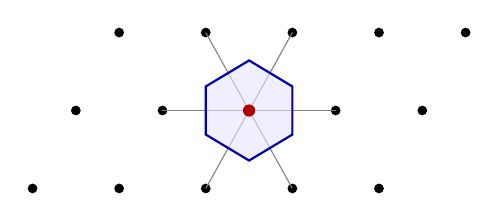
\begin{tikzpicture}[scale=1.1]
  \foreach \i in {-2,...,2} \foreach \j in {-1,0,1} \fill ({\i+0.5*\j},{0.9*\j}) circle (1.6pt);
  \foreach \p in {(1,0),(-1,0),(0.5,0.9),(-0.5,0.9),(0.5,-0.9),(-0.5,-0.9)} \draw[gray] (0,0) -- \p;
  \draw[thick,blue!70!black,fill=blue!10,fill opacity=0.6]
    (0.5,0.2778) -- (0,0.5778) -- (-0.5,0.2778) -- (-0.5,-0.2778) -- (0,-0.5778) -- (0.5,-0.2778) -- cycle;
  \fill[red!70!black] (0,0) circle (2pt);
\end{tikzpicture}
\caption{Malla de Wigner--Seitz en una red 2D (hexágono sombreado).}
\end{figure}

Esta malla de W--S en la red recíproca se llama \textbf{primera zona de Brillouin} (contiene todos los diferentes estados).

\subsection{Tipos de cristales según la fuerza interatómica}
\begin{enumerate}
  \item \textbf{Cristales moleculares:} la fuerza interatómica (o intermolecular) es pequeña (como las fuerzas de Van der Waals).
  \item \textbf{Cristales covalentes:} enlace covalente. Ej.: Si, Ge.
  \item \textbf{Cristales iónicos:} enlace iónico. Ej.: NaCl.
  \item \textbf{Cristales metálicos:} la fuerza entre los e$^-$ libres y los iones (+) (átomos que han perdido e$^-$). Son los metales.
\end{enumerate}
% ============================================================
\section{Modelo del electrón libre \pags{59--62}}
% ============================================================

\textbf{Estudio de los metales:} de cada átomo se desprenden los e$^-$ de los últimos niveles atómicos (electrones de valencia),
débilmente ligados al núcleo. Quedan iones (+) fijos y electrones libres moviéndose entre ellos.

Hay propiedades que se pueden explicar con el modelo clásico (conductividad, otras). Pero hay otras que no (capacidad
calorífica, otras).

\subsection{Modelo de Drude (el modelo clásico más simple)}
Tomemos un conductor de forma cilíndrica. Sin campo, los e$^-$ se mueven al azar: el flujo neto de carga a través de una
sección $S$ será cero.

Aplicamos un campo eléctrico $\vec E$ $\rightarrow$ hay fuerza $\rightarrow$ aceleración. Los e$^-$ libres aceleran, chocan con los iones
de la red y pierden la velocidad ganada. Nuevamente se aceleran, nuevamente chocan\ldots\ En promedio, se establece un MRU
con $\vec v_d$ (velocidad de arrastre).

En $\Delta t$ logran atravesar $S$ todos los e$^-$ libres que están en el volumen $(S\,v_d\,\Delta t)$:
\[
\Delta N=\#e=n\,(S\,v_d\,\Delta t),\qquad n:\ \text{concentración de electrones}\ \left(\frac{\#\ \text{electrones}}{\text{volumen}}\right)
\]
\[
i=\frac{(\Delta N)\,e}{\Delta t}=\frac{nSv_d\,\Delta t\,e}{\Delta t}\ \Rightarrow\ \boxed{i=nev_dS}
\]
Densidad de corriente:
\[
|\vec J|=\frac iS=\frac{nev_dS}{S}=nev_d,\qquad \vec J=-ne\,\vec v_d
\]
\textbf{Conductividad:} relación entre $\vec J$ (efecto) y $\vec E$ (causa). Experimentalmente $J\sim E$:
\[
\vec J=\sigma\vec E
\]
Analogía entre el movimiento de un electrón libre y una bolita en un fluido: los choques $\sim$ fuerza de viscosidad ($-b\vec v_d$).
\[
-e\vec E-b\vec v_d=0\ \Rightarrow\ \vec v_d=-\frac eb\vec E,\qquad \vec v_d=-\mu\vec E\quad(\mu:\ \text{movilidad de los e}^-\text{ libres})
\]
Por otros estudios, $b=m/\tau$:
\begin{itemize}
  \item $m$: masa del e$^-$.
  \item $\tau$: tiempo de recorrido libre medio (tiempo de relajación).
  \item $l$: longitud de recorrido libre medio; \ $l/\tau=u$ (velocidad de agitación térmica).
\end{itemize}
\[
\vec v_d=\frac{-e\vec E}{m/\tau}=-\frac{e\tau}{m}\vec E\ \Rightarrow\ \mu=\frac{e\tau}{m}
\]
\[
\vec J=-ne\left(-\frac{e\tau}{m}\vec E\right)=\frac{ne^2\tau}{m}\vec E,\qquad
\boxed{\sigma=ne\mu=\frac{ne^2\tau}{m}}\ \ (\text{conductividad})
\]

\subsection{Modelo del e$^-$ libre cuántico}
\begin{itemize}
  \item Los e$^-$ libres son partículas cuánticas: tienen propiedad ondulatoria (ecuación de Schrödinger).
  \item Los e$^-$ libres cumplen el principio de exclusión de Pauli.
\end{itemize}
Podemos tomar al metal como una caja 3D (o su proyección, caja 1D). Cada rayita (nivel) está determinada por los números
cuánticos $n_1,n_2,n_3,m_s$; los electrones llenan los niveles desde abajo.

\textbf{$\Ep_F$: energía de Fermi} (a la $T$ de 0~K, es la energía del e$^-$ más energético).

\textbf{Distribución del número de partículas por $E$:} a $T=0$~K, todos los niveles hasta $\Ep_F$ están ocupados y ninguno por encima.

A una temperatura $T>0$ (la temperatura ha pasado de 0 a $T$), la energía cinética promedio aumenta $\rightarrow$ cada e$^-$ aumenta
su energía en $\tfrac32k_BT$ \ ($k_B$: constante de Boltzmann):
\[
\frac32\cdot\frac{1{,}38\times10^{-23}\times300}{1{,}6\times10^{-19}}\approx0{,}038\ \text{eV}
\]
$\Ep_F$ se mide en unidades de eV, así que solo los e$^-$ muy cerca de $\Ep_F$ (dentro de $\sim0{,}03$ eV) pueden subir a niveles libres.

\subsection{Función de distribución de Fermi--Dirac}
\[
\boxed{f(E)=\frac{1}{e^{(E-\Ep_F)/k_BT}+1}}
\]
$f(E)$: probabilidad de que los estados con energía $E$ estén ocupados.

\begin{figure}[H]
\centering
\begin{tikzpicture}
\begin{axis}[width=8cm,height=4.5cm,axis lines=left,xlabel={$E$},ylabel={$f(E)$},
  xtick={3},xticklabels={$\Ep_F$},ytick={0.5,1},yticklabels={{0{,}5},1},xmin=0,xmax=6,ymin=0,ymax=1.2,samples=200,domain=0:6,
  every axis x label/.style={at={(ticklabel* cs:1)},anchor=west},
  every axis y label/.style={at={(ticklabel* cs:1)},anchor=south}]
  \addplot[thick,dashed,gray] coordinates {(0,1) (3,1) (3,0) (6,0)};
  \addplot[thick,blue!70!black] {1/(exp((x-3)/0.3)+1)};
  \draw[dotted] (axis cs:0,0.5) -- (axis cs:3,0.5);
  \node[font=\small,gray] at (axis cs:1.3,1.1) {$T=0$ K};
  \node[font=\small,blue!70!black] at (axis cs:4.6,0.35) {$T>0$ K};
\end{axis}
\end{tikzpicture}
\caption{Función de Fermi--Dirac: escalón a $T=0$ K; a $T>0$ K cae suavemente y vale 0,5 en $E=\Ep_F$.}
\end{figure}

\subsection{Capacidad calorífica}
Cuando pasa de 0 a $T$, $\Delta T=T-0=T$.
\[
Q=C\,\Delta T\ \rightarrow\ \text{incremento de energía }\left(\tfrac32k_B\Delta T\right);\qquad N\text{ partículas: }\tfrac32k_B\Delta T\,N
\]
\[
Q=C\,\Delta T=\frac32k_B\Delta T\,N\ \Rightarrow\ C=\frac32k_BN
\]
Pero, experimentalmente: $C\approx\dfrac{1}{100}\left(\dfrac32k_BN\right)$. Con el modelo cuántico, solo incrementan su energía los
que están cerca a $\Ep_F$.

\subsection{Densidad de estados}
\[
g(E)=\frac{\#\ \text{estados con energías entre }E\text{ y }E+dE}{dE}
\]
Modelo: caja cúbica de lado $L$ (volumen $L^3$):
\[
\varphi=C\sen\frac{n_1\pi}{L}x\,\sen\frac{n_2\pi}{L}y\,\sen\frac{n_3\pi}{L}z,\qquad
E=\frac{\hbar^2\pi^2}{2mL^2}(n_1^2+n_2^2+n_3^2)=\frac{\hbar^2}{2m}(k_x^2+k_y^2+k_z^2)
\]
donde $k_x=\dfrac{n_1\pi}{L}$, $k_y=\dfrac{n_2\pi}{L}$, $k_z=\dfrac{n_3\pi}{L}$.

\textbf{Espacio-$\vec k$:} cada punto es un estado; la energía $E$ corresponde a una esfera, y entre $E$ y $E+dE$ hay un cascarón.

\begin{figure}[H]
\centering
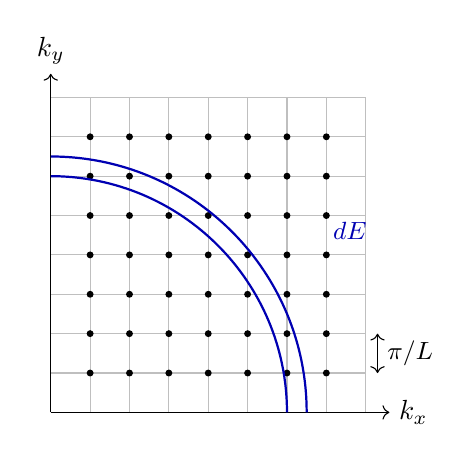
\begin{tikzpicture}[scale=0.5]
  \draw[step=1,gray!50] (0,0) grid (8,8);
  \foreach \x in {1,...,7} \foreach \y in {1,...,7} \fill (\x,\y) circle (2.5pt);
  \draw[->] (0,0) -- (8.6,0) node[right]{$k_x$};
  \draw[->] (0,0) -- (0,8.6) node[above]{$k_y$};
  \draw[thick,blue!70!black] (6,0) arc (0:90:6);
  \draw[thick,blue!70!black] (6.5,0) arc (0:90:6.5);
  \node[font=\small,blue!70!black] at (7.6,4.6) {$dE$};
  \draw[<->] (8.3,1) -- (8.3,2) node[midway,right,font=\small]{$\pi/L$};
\end{tikzpicture}
\caption{Espacio-$\vec k$ en 2 dimensiones: cada celda de lado $\pi/L$ contiene un estado.}
\end{figure}

\begin{itemize}
  \item En 2 dimensiones: número de puntos $=$ número de celdas $\rightarrow$ N.~est. $=\dfrac{\text{área}}{\text{área de una celda}}=\dfrac{\text{área}}{(\pi/L)^2}$.
  \item En 3 dimensiones: N.~est. $=\dfrac{\text{volumen}}{\text{volumen de una celda}}=\dfrac{\text{volumen del cascarón}}{(\pi/L)^3}$.
\end{itemize}
\[
g(E)=\frac{4\pi|\vec k|^2\,d|\vec k|}{dE\,(\pi/L)^3}\cdot\frac18\cdot2
\]
($\tfrac18$: 1.\textsuperscript{er} octante, porque $n_1,n_2,n_3$ son positivos en la caja; $\times2$: spin.)
\[
\frac{2mE}{\hbar^2}=k_x^2+k_y^2+k_z^2=|\vec k|^2\ \xrightarrow{\text{diferenciamos}}\ \frac{2m}{\hbar^2}\,dE=2|\vec k|\,d|\vec k|
\]
\[
g(E)=\frac{4\pi\frac{\sqrt{2mE}}{\hbar}\cdot\frac{m\,dE}{\hbar^2}}{dE\,(\pi/L)^3}\cdot\frac14
=\frac{1}{2\pi^2}\left(\frac{2m}{\hbar^2}\right)^{3/2}E^{1/2}\,L^3
\ \Rightarrow\
\boxed{g(E)=\frac{1}{2\pi^2}\left(\frac{2m}{\hbar^2}\right)^{3/2}E^{1/2}\,V}
\]

\begin{obs}
En la línea «diferenciamos» el cuaderno escribe $2m/\hbar$ en vez de $2m/\hbar^2$ (lo mismo luego en $dN(E)$); el resultado final sí
usa $\hbar^2$ y es correcto.
\end{obs}

Por unidad de volumen:
\[
\boxed{\mathcal D(E)=\frac{g(E)}{V}=\frac{1}{2\pi^2}\left(\frac{2m}{\hbar^2}\right)^{3/2}E^{1/2}}
\]

\textbf{Otra forma: espacio de los números cuánticos.} Cada estado ocupa un cubito de volumen $1\cdot1\cdot1$, y la energía $E$ es una
esfera de radio $R$:
\[
n_1^2+n_2^2+n_3^2=\frac{2mEL^2}{\hbar^2\pi^2}=R^2
\]
$N(E)$: número de estados con energías desde 0 hasta $E$:
\[
N(E)=\frac{\text{volumen esfera}}{1\cdot1\cdot1}\cdot\frac18\cdot2=\frac{\frac43\pi\left(\frac{2mEL^2}{\hbar^2\pi^2}\right)^{3/2}}{1\cdot1\cdot1}\cdot\frac18\cdot2
\]
Diferenciamos:
\[
dN(E)=\frac{1}{3\pi^2}\left(\frac{2m}{\hbar^2}\right)^{3/2}L^3\,\frac32E^{1/2}\,dE,\qquad g(E)=\frac{dN(E)}{dE}
\]
($dN(E)$: número de estados con energías entre $E$ y $E+dE$.)

\subsection{Ejemplo: estados por volumen entre 0 y $\Ep_F$}
Halle el número de estados/volumen con energías entre 0 y $\Ep_F$.
\[
\text{N. est.}=\int_0^{\Ep_F}\mathcal D\,dE=\int_0^{\Ep_F}\frac{1}{2\pi^2}\left(\frac{2m}{\hbar^2}\right)^{3/2}E^{1/2}\,dE
=\frac23\cdot\frac{1}{2\pi^2}\left(\frac{2m}{\hbar^2}\right)^{3/2}\Ep_F^{3/2}
=\frac{1}{3\pi^2}\left(\frac{2m}{\hbar^2}\right)^{3/2}\Ep_F^{3/2}
\]
A $T=0$ K todos esos estados están llenos (N.~est. $=n$), así que:
\[
\boxed{\Ep_F=\frac{\hbar^2}{2m}\,(3\pi^2n)^{2/3}}
\]
\[
\#\ \text{estados entre }E_1\text{ y }E_2=\int_{E_1}^{E_2}\mathcal D\,dE,\qquad
\#\ \text{electrones entre }E_1\text{ y }E_2=\int_{E_1}^{E_2}f(E)\,\mathcal D(E)\,dE
\]

\begin{obs}
En el cuaderno la última integral también se rotula «N. estados», pero al llevar $f(E)$ cuenta electrones (estados ocupados),
como dice el título.
\end{obs}

% ============================================================
\section{Efecto Hall \pags{62}}
% ============================================================

Aparición de un voltaje ($V_H$) en forma transversal a la corriente, en un conductor, al aplicar un campo $\vec B$.

\begin{figure}[H]
\centering
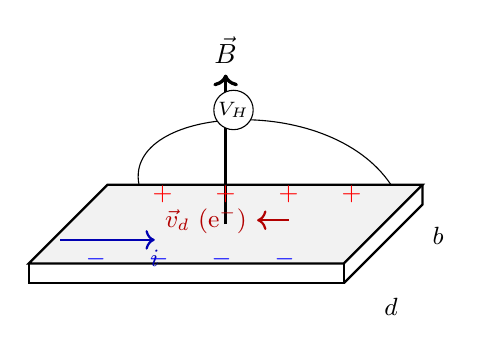
\begin{tikzpicture}[scale=1]
  \draw[thick,fill=gray!10] (0,0) -- (4,0) -- (5,1) -- (1,1) -- cycle;
  \draw[thick] (0,0) -- (0,-0.25) -- (4,-0.25) -- (4,0); \draw[thick] (4,-0.25) -- (5,0.75) -- (5,1);
  \draw[->,very thick] (2.5,0.5) -- (2.5,2.4) node[above]{$\vec B$};
  \draw[->,thick,blue!70!black] (0.4,0.3) -- (1.6,0.3) node[below,font=\small]{$i$};
  \draw[->,thick,red!70!black] (3.3,0.55) -- (2.9,0.55) node[left,font=\small]{$\vec v_d$ (e$^-$)};
  \foreach \x in {0.8,1.6,...,3.6} \node[font=\small,blue] at (\x+0.05,0.05) {$-$};
  \foreach \x in {1.8,2.6,...,4.6} \node[font=\small,red] at (\x-0.1,0.88) {$+$};
  \draw (1.4,1) .. controls (1.2,2) and (3.8,2.2) .. (4.6,1);
  \draw[fill=white] (2.6,1.95) circle (0.25) node{\scriptsize $V_H$};
  \node[font=\small] at (4.6,-0.55) {$d$}; \node[font=\small] at (5.2,0.35) {$b$};
\end{tikzpicture}
\caption{Efecto Hall: los portadores se desvían y aparece el voltaje transversal $V_H$.}
\end{figure}

Experimentalmente:
\[
V_H\sim\frac{iB}{d}\ \Rightarrow\ V_H=R_H\,\frac{iB}{d}
\]
Equilibrio entre la fuerza magnética ($-e\vec v_d\times\vec B$) y la eléctrica ($-e\vec E_H$), con $i=nev_d(bd)$:
\[
ev_dB=eE_H=e\left(\frac{V_H}{b}\right)\ \Rightarrow\ \frac{i}{nebd}\cdot B=\frac{V_H}{b}\ \Rightarrow\ \boxed{V_H=\frac{1}{ne}\,\frac{iB}{d}}
\]
Una aplicación: determinar $n$.

\begin{obs}
El coeficiente de Hall es $R_H=1/(nq)$; para electrones ($q=-e$) es negativo. El signo de $V_H$ permite saber si los portadores
son electrones o huecos.
\end{obs}

% ============================================================
\section{Teoría de bandas \pags{62--64}}
% ============================================================

\textbf{Ecuación de Schrödinger para un cristal:} $\hat H\varphi=E\varphi$
\[
\Bigg\{\sum_i-\frac{\hbar^2}{2m_i}\nabla_i^2+\sum_\alpha-\frac{\hbar^2}{2M_\alpha}\nabla_\alpha^2
+\underbrace{\frac12\sum_{i\neq j}\frac{e^2}{4\pi\varepsilon_0r_{ij}}}_{U_e}
+\underbrace{U_n}_{\substack{\text{núcleos}\\ \text{entre sí}}}+\underbrace{U}_{\substack{\text{núcleos}\\ \text{con e}^-}}\Bigg\}
\varphi(\vec r_1,\vec r_2,\ldots,\vec R_1,\vec R_2,\ldots)=E\varphi
\]
(El $\tfrac12$ evita contar dos veces cada par: $r_{12}$ y $r_{21}$.)

\subsection{Aproximaciones}
\textbf{Aproximación adiabática:} considera a los núcleos en reposo; $U_K=\text{const}=0$ en particular.
\[
\left\{\sum_i-\frac{\hbar^2}{2m_i}\nabla_i^2+U_e+U\right\}\varphi(\vec r_1,\vec r_2,\ldots)=E\varphi(\vec r_1,\vec r_2,\ldots)
\]
\textbf{Aproximación de valencia:} se consideran solo los e$^-$ de valencia y los iones.

\textbf{Aproximación monoelectrónica:}
\[
\frac12\sum_{i\neq j}\frac{e^2}{4\pi\varepsilon_0r_{ij}}\ \rightarrow\ \sum_i\Omega_i(\vec r_i)
\]
$\Omega_i$: energía potencial del electrón «$i$» en el campo del resto de electrones:
\[
\left(\frac{e^2}{4\pi\varepsilon_0r_{12}}+\frac{e^2}{4\pi\varepsilon_0r_{13}}+\frac{e^2}{4\pi\varepsilon_0r_{14}}+\frac{e^2}{4\pi\varepsilon_0r_{23}}+\cdots\right)\rightarrow\Omega_1+\Omega_2+\cdots
\]
También $U\rightarrow\sum_iV_i(\vec r_i)$; $V_i$: energía potencial del e$^-$ «$i$» en el campo de todos los núcleos.
\[
\left\{\sum_i-\frac{\hbar^2}{2m_i}\nabla_i^2+\sum_i\Omega_i(\vec r_i)+\sum_iV_i(\vec r_i)\right\}\varphi=E\varphi
\ \Rightarrow\
\Bigg\{\sum_i\underbrace{\left(-\frac{\hbar^2}{2m_i}\nabla_i^2+\Omega_i+V_i\right)}_{\hat H_i}\Bigg\}\varphi=E\varphi
\]
\[
\left\{\sum_i\hat H_i\right\}\varphi(\vec r_1,\vec r_2,\ldots)=E\varphi(\vec r_1,\vec r_2,\ldots)
\]

\subsection{Relación de dispersión $E(\vec k)$}
Funciones de onda atómicas centradas en átomos vecinos $g$ y $g'$, separados por $\vec q_g=\vec R_g-\vec R_{g'}$.

\textbf{Ejemplo: red SC. Halle $E(\vec k)$ (relación de dispersión).}
\[
E=E_a+C+A\sum_{\text{vecinos}}e^{i\vec k\cdot\vec q_g}
\]
Vecinos: $\vec q_1=a\ii$, $\vec q_2=-a\ii$, $\vec q_3=a\jj$, $\vec q_4=-a\jj$, $\vec q_5=a\kk$, $\vec q_6=-a\kk$; \
$\vec k=k_x\ii+k_y\jj+k_z\kk$.
\[
E=E_a+C+A\left(e^{ik_xa}+e^{-ik_xa}+e^{ik_ya}+e^{-ik_ya}+\cdots\right)=E_a+C+2A(\cos k_xa+\cos k_ya+\cos k_za)
\]

\textbf{Banda S:} $A<0$. En 1 dimensión, $E=E_a+C+2A\cos k_xa$:

\begin{figure}[H]
\centering
\begin{tikzpicture}
\begin{axis}[width=10cm,height=5cm,axis lines=middle,xlabel={$k_x$},ylabel={$E$},
  xtick={-3.1416,3.1416},xticklabels={$-\pi/a$,$\pi/a$},ytick=\empty,xmin=-6,xmax=6,ymin=-1.4,ymax=1.6,samples=200,
  every axis x label/.style={at={(ticklabel* cs:1)},anchor=west},
  every axis y label/.style={at={(ticklabel* cs:1)},anchor=south}]
  \addplot[thick,blue!70!black,domain=-3.1416:3.1416] {-cos(deg(x))};
  \addplot[thick,dashed,blue!70!black,domain=-5.8:-3.1416] {-cos(deg(x))};
  \addplot[thick,dashed,blue!70!black,domain=3.1416:5.8] {-cos(deg(x))};
  \draw[dashed,gray] (axis cs:-3.1416,-1.3) -- (axis cs:-3.1416,1.3);
  \draw[dashed,gray] (axis cs:3.1416,-1.3) -- (axis cs:3.1416,1.3);
  \draw[<->] (axis cs:-3.1416,-1.25) -- (axis cs:3.1416,-1.25) node[midway,below,font=\small]{1.\textsuperscript{ra} zona de Brillouin};
\end{axis}
\end{tikzpicture}
\caption{Banda S en 1D: mínimo en $k_x=0$ y máximos en $\pm\pi/a$.}
\end{figure}

\textbf{Banda P:} la curva tiene la forma invertida (máximo en $k=0$).

\begin{obs}
Este es el modelo de enlace fuerte (\emph{tight binding}): $E_a$ es la energía del nivel atómico, $C$ un corrimiento y $A$ la integral de
solapamiento con los vecinos. El ancho de la banda en 3D es $12|A|$.
\end{obs}

Partícula libre (para comparar): $E=E_K=\dfrac{p^2}{2m}=\dfrac{(\hbar k)^2}{2m}$.

\subsection{Masa efectiva ($m^*$)}
Velocidad (en 1 dimensión):
\[
v_g=\frac1\hbar\frac{dE}{dk}
\]
Aceleración:
\[
a=\frac{dv_g}{dt}=\frac{dv_g}{dk}\cdot\frac{dk}{dt}=\frac{d}{dk}\left(\frac1\hbar\frac{dE}{dk}\right)\cdot\frac F\hbar,\qquad
F=\frac{dp}{dt}=\frac{d}{dt}(\hbar k)=\hbar\frac{dk}{dt}
\]
\[
\Rightarrow\ a=\underbrace{\frac{1}{\hbar^2}\frac{d^2E}{dk^2}}_{1/m^*}\cdot F
\qquad\Rightarrow\qquad
\boxed{m^*=\frac{\hbar^2}{d^2E/dk^2}}
\]
El electrón siente fuerzas internas (de la red) y externas; con $m^*$ se escribe $F_{\text{ext}}=m^*a$, como si solo existiera la fuerza
externa. Puede resultar $m^*<m$.

\subsection{Hueco}
Cerca del tope de una banda casi llena, $E(k)$ tiene un máximo. Por simetría, a cada estado $\vec k$ le corresponde $-\vec k=\vec k\,'$
con velocidad $-\vec v=\vec v\,'$.
\[
\vec p=m\vec v=\hbar\vec k,\qquad \vec J=ne\vec v_d=(1+1+1+\cdots)q\vec v,\qquad \vec J=\sum q_i\vec v_i=-e\sum\vec v_i
\]
Con campo:
\[
-e\vec E=\hbar\frac{\Delta\vec k}{\Delta t}\ \rightarrow\ \Delta\vec k
\]
Todos los estados se desplazan $\Delta\vec k$ en el espacio-$k$; en una banda llena la suma de velocidades sigue siendo cero, así que
solo los estados vacíos (huecos) dan corriente neta.

\begin{obs}
El hueco se comporta como una partícula de carga $+e$ y masa efectiva positiva (cerca del tope de la banda, $d^2E/dk^2<0$, de modo que
la $m^*$ del electrón ahí es negativa).
\end{obs}

% ============================================================
\section{Semiconductores \pags{64}}
% ============================================================

Diagramas de bandas a $T=0$ K (BC: banda de conducción; BV: banda de valencia):

\begin{figure}[H]
\centering
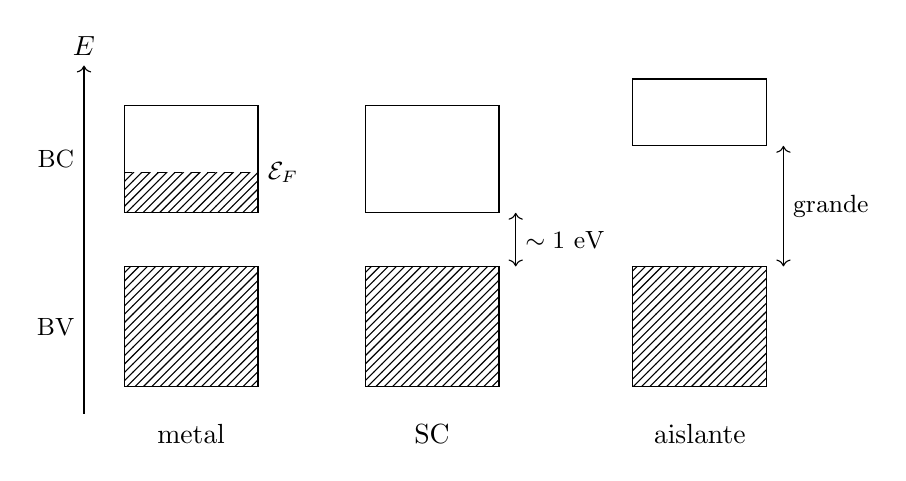
\begin{tikzpicture}[scale=0.85]
  \draw[->] (-0.6,0) -- (-0.6,5.2) node[above]{$E$};
  % metal
  \draw (0,3) rectangle (2,4.6); \fill[pattern=north east lines] (0,3) rectangle (2,3.6);
  \draw[dashed] (0,3.6) -- (2,3.6) node[right,font=\small]{$\Ep_F$};
  \draw (0,0.4) rectangle (2,2.2); \fill[pattern=north east lines] (0,0.4) rectangle (2,2.2);
  \node[left,font=\small] at (-0.6,3.8) {BC}; \node[left,font=\small] at (-0.6,1.3) {BV};
  \node at (1,-0.3) {metal};
  % semiconductor
  \begin{scope}[xshift=3.6cm]
  \draw (0,3) rectangle (2,4.6);
  \draw (0,0.4) rectangle (2,2.2); \fill[pattern=north east lines] (0,0.4) rectangle (2,2.2);
  \draw[<->] (2.25,2.2) -- (2.25,3) node[midway,right,font=\small]{$\sim1$ eV};
  \node at (1,-0.3) {SC};
  \end{scope}
  % aislante
  \begin{scope}[xshift=7.6cm]
  \draw (0,4) rectangle (2,5);
  \draw (0,0.4) rectangle (2,2.2); \fill[pattern=north east lines] (0,0.4) rectangle (2,2.2);
  \draw[<->] (2.25,2.2) -- (2.25,4) node[midway,right,font=\small]{grande};
  \node at (1,-0.3) {aislante};
  \end{scope}
\end{tikzpicture}
\caption{Metal, semiconductor y aislante a $T=0$ K (lo rayado está ocupado).}
\end{figure}

Conductividad con dos tipos de portadores (electrones $n$ y huecos $p$):
\[
\boxed{\sigma=\sigma_n+\sigma_p=\frac{ne^2\tau_n}{m_n^*}+\frac{pe^2\tau_p}{m_p^*}}
\]

\begin{figure}[H]
\centering
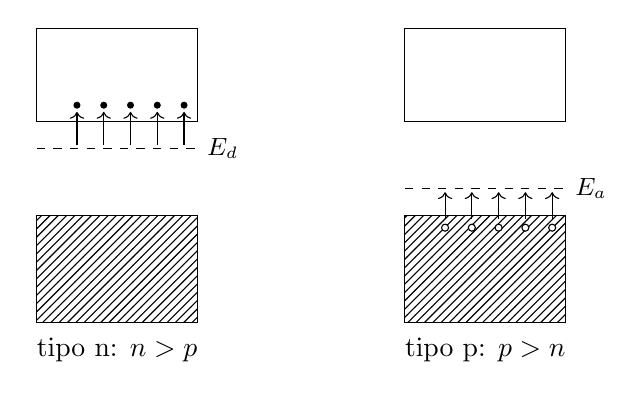
\begin{tikzpicture}[scale=0.85]
  % tipo n
  \draw (0,3) rectangle (2.4,4.4); \draw (0,0) rectangle (2.4,1.6); \fill[pattern=north east lines] (0,0) rectangle (2.4,1.6);
  \draw[dashed] (0,2.6) -- (2.4,2.6) node[right,font=\small]{$E_d$};
  \foreach \x in {0.6,1.0,...,2.2} {\draw[->,thin] (\x,2.65) -- (\x,3.15); \fill (\x,3.25) circle (1.5pt);}
  \node at (1.2,-0.4) {tipo n: $n>p$};
  % tipo p
  \begin{scope}[xshift=5.5cm]
  \draw (0,3) rectangle (2.4,4.4); \draw (0,0) rectangle (2.4,1.6); \fill[pattern=north east lines] (0,0) rectangle (2.4,1.6);
  \draw[dashed] (0,2.0) -- (2.4,2.0) node[right,font=\small]{$E_a$};
  \foreach \x in {0.6,1.0,...,2.2} {\draw[->,thin] (\x,1.55) -- (\x,1.95); \draw[fill=white] (\x,1.42) circle (1.5pt);}
  \node at (1.2,-0.4) {tipo p: $p>n$};
  \end{scope}
\end{tikzpicture}
\caption{Niveles de impurezas: donadoras ($E_d$, bajo la BC) y aceptadoras ($E_a$, sobre la BV).}
\end{figure}

\textbf{Tipo n (impurezas donadoras):} nivel $E_d$ justo debajo de la BC; los e$^-$ de las impurezas pasan fácilmente a la BC
$\rightarrow$ $n>p$.

\textbf{Tipo p (impurezas aceptadoras):} nivel $E_a$ justo encima de la BV; los e$^-$ de la BV pasan a $E_a$ y dejan huecos
$\rightarrow$ $p>n$.

Al final, el cuaderno deja el esquema de una unión p--n conectada a una batería, con una zona central de ancho $d$, y una red con átomos
de impureza (sin texto).

\begin{obs}
La zona de ancho $d$ de la unión p--n es la región de agotamiento (o de carga espacial). Con polarización directa se estrecha y conduce;
con polarización inversa se ensancha y casi no pasa corriente.
\end{obs}

\end{document}
